%%%%%%%%%%%%%%%%%%%%%%%%%%%%%%%%%%%%%%%%
% PDF compatibility code. 
\makeatletter
\newif\ifpdflatex@
\ifx\pdftexversion\@undefined
\pdflatex@false
%\message{Not using pdf}
\else
\pdflatex@true
%\message{Using pdf}
\fi

\newcommand{\latexorpdf}[2]{
  \ifpdflatex@ #2
  \else #1
  \fi
}

\makeatother

#ifdef A4Format
\newcommand{\pformat}{a4paper}
#endif A4Format
#ifdef LetterFormat
\newcommand{\pformat}{letterpaper}
#endif LetterFormat

%%%%%%%%%%%%%%%%%%%%%%%%%%%%%%%%%%%%%%%%

\latexorpdf{
\documentclass[\pformat,12pt]{article}
}{
\documentclass[\pformat,pdftex,12pt]{article}
}

\usepackage[dvipdfm]{graphicx, color}
\usepackage[dvipdfm,bookmarks=true,bookmarksnumbered=true,colorlinks,plainpages=true]{hyperref}

\usepackage{toolbox}
\usepackage{vdmsl-2e}
\usepackage{makeidx}
\usepackage{alltt}
%\usepackage{graphics}
%\usepackage{verbatim}
\usepackage{ifthen}
\usepackage{verbatimfiles}
%\usepackage{color}
\usepackage{longtable}
%\usepackage{path}
\usepackage{here}

\graphicspath{{figures/}}
\def\seename{$\Rightarrow$}

\makeindex

% The use of VDMSL/VDMPP ifdef's have basicly been exchanged with the
% use of LaTeX ifthenelse's.  For this two LaTeX boolean value VDMSL and
% VDMpp have been defined  (Lowercase p's are used to avoid conflict with
% the VDMPP environment variable.  The typical use are:
%   \ifthenelse{\boolean{VDMsl}}{vdmsl-text}{vdmpp-text}
%   \ifthenelse{\boolean{VDMsl}}{vdmsl-text}{}
%   \ifthenelse{\boolean{VDMpp}}{vdmpp-text}{}
% The advantage of this as opposed to ifdef's is that within a general
% paragraph specific VDM-SL and VDM++ parts can be distinguished without
% problematic empty lines.
% 
% The values are initialised such that exactly one of the values is true
% and the other is false.  This should hopefully avoid strange behaviour
% due to possible preprossing errors.  The default case is VDM-SL.
\newboolean{VDMsl}
\setboolean{VDMsl}{true}
\newboolean{VDMpp}
\setboolean{VDMpp}{false}
#ifdef VDMSL
\setboolean{VDMsl}{true}
\setboolean{VDMpp}{false}
#endif VDMSL
#ifdef VDMPP
\setboolean{VDMpp}{true}
\setboolean{VDMsl}{false}
#endif VDMPP


\def\vdmsl{{\small VDM-SL}}
\def\vdmpp{{\small VDM}$^{++}$}
#ifdef VDMSL
\newcommand{\vdmslpp}{VDM-SL}
\newcommand{\vdmslppEm}{VDM-SL}
\newcommand{\ToolboxName}{VDM-SL Toolbox}
\newcommand{\Toolbox}{Toolbox}
\newcommand{\toolbox}{Toolbox}
\newcommand{\vdmde}{vdmde}
\newcommand{\vdmgde}{vdmgde}
\newcommand{\vdmhome}{vdmhome}
\newcommand{\vdmdeNineteen}{vdmde-19}
\newcommand{\vdmdeNineteenEl}{vdmde-19.el}
\newcommand{\VdmSlPp}{\VdmSl}
#endif VDMSL
#ifdef VDMPP
\newcommand{\vdmslpp}{VDM++}
\newcommand{\vdmslppEm}{VDM\/++}
\newcommand{\ToolboxName}{VDM++ Toolbox}
\newcommand{\Toolbox}{Toolbox}
\newcommand{\toolbox}{toolbox}
\newcommand{\vdmde}{vppde}
\newcommand{\vdmgde}{vppgde}
\newcommand{\vdmhome}{vpphome}
\newcommand{\vdmdeNineteen}{vppde-19}
\newcommand{\vdmdeNineteenEl}{vppde-19.el}
\DeclareRobustCommand{\VdmSlPp}{VDM++-\VdmSl}
#endif VDMPP

\newcommand{\guicmd}[1]{{\sf #1}}

\begin{document}
#ifdef VDMSL
\vdmtoolsmanualscsk{The VDM-SL to C++ Code Generator}{2.0}
#else
\vdmtoolsmanualscsk{The VDM++ to C++ Code Generator}{2.0}
#endif //VDMPP


\newcommand{\tcg}{the Code Generator}
\newcommand{\Tcg}{The Code Generator}

#ifdef VDMPP
\newcommand{\libmancite}{\cite{LibMan-SCSK}}
\newcommand{\langmancite}{\cite{LangManPP-SCSK}}
%\newcommand{\VDM}{VDM\raisebox{-0.6ex}{++}}
\newcommand{\VDM}{VDM++}
\newcommand{\cg}{VDM++ to C++ Code Generator}
%\newcommand{\toolbox}{VDM$^{++}$ Toolbox}
\newcommand{\MCL}{VDM C++ Library}
\newcommand{\CGBase}{\texttt{CGBase}}
#endif VDMPP

#ifdef VDMSL
\newcommand{\libmancite}{\cite{LibMan-SCSK}}
\newcommand{\langmancite}{\cite{LangMan-SCSK}}
\newcommand{\cg}{VDM-SL to C++ Code Generator}
%\newcommand{\toolbox}{VDM-SL Toolbox}
\newcommand{\MCL}{VDM C++ Library}
\newcommand{\VDM}{VDM-SL}
#endif VDMSL


%Installation should be described in the Installation document.
\section{Introduction}


The \cg\ supports automatic generation of C++ code from \VDM\ 
specifications. This way, \tcg\ provides you with a fast way of
implementing applications based on \VDM\ specifications.

 \Tcg\ is an add-on
feature to the \ToolboxName{}. Its installation is described in the document
\ifthenelse{\boolean{VDMsl}}{\cite{InstallMan-SCSK}}{\cite{InstallPPMan-SCSK}}.
The following text is an extension to the {\em VDMTools User Manual (\VDM{})}
\ifthenelse{\boolean{VDMsl}}{\cite{UserMan-SCSK}}{\cite{UserManPP-SCSK}} and it
gives you an introduction to 
the \cg{}.

The Code Generator supports approximately 95\% of all the \VDM\ constructs.
As a supplement, the user is given the possibility of substituting parts of
the generated code with handwritten code. 

This manual is structured in the following way:

Section~\ref{invoking} lists the requirements that the \VDM\ specification
has to satisfy in order to generate correct C++ code.
Moreover, this section describes how to invoke the \cg{} from the
 \ToolboxName{}. Finally, the code generated C++ files will be described.

Section~\ref{interfacing} guides you in the writing of 
an interface to the generated C++ code and it explains how to interface
handwritten code to it. Furthermore, it will be explained how
to compile, link and run the C++ code.  

Section~\ref{sec:unsupported} summarizes the \VDM\ constructs not
supported by \tcg{}.

Section~\ref{sec:relation} gives a detailed description of the structure
of the generated C++ code. In addition, it explains the relation between \VDM\ and
C++ data types, and it describes some of the design decisions made, when
developing the \cg{}, including the name conventions used. This
section should be studied intensively before using \tcg\
professionally.


\section{Invoking the Code Generator}\label{invoking}


%Type \path+codegen+
%and the specification is type checked and the files \path+DefaultMod.h+
%and \path+DefaultMod.cc+ are generated (On Windows platforms the
%implementation file is named \path+DefaultMod.cpp+).

%A detailed description of the usage of the \cg{} is given in the
%Sections 4 and 5 in {\em User Manual for the IFAD \VDM{} Toolbox\/}
%\cite{UserMan}.
%#endif VDMSL

To get started using \tcg\ you should write a \VDM\ specification in
one or several files. In the distribution of the \Toolbox\, a
specification of different sorting algorithms is included. This
specification will be used in the following in order to describe the
use of \tcg{}. This specification is described in
\ifthenelse{\boolean{VDMsl}}{\cite{SortEx-SCSK}}{\cite{SortExpp-SCSK}}.  It is
recommended that you go through the described steps on your own
computer. In order to do so, copy the directory
\path+vdmhome/examples/sort+ and \path+cd+ to it.

Before generating C++ code, it has to be ensured, that the \VDM\ 
specification satisfies the necessary requirements. The requirements
in question will be described in Section~\ref{requirements}.  In
Section~\ref{gui} and ~\ref{commandline} it will be explained how to
generate C++ code using the \ToolboxName\ from the graphical
interface and from the command line.
In Section~\ref{sec:cppfiles} the code generated C++ files will be described.

\subsection{Requirements for Generating Code}\label{requirements}

#ifdef VDMPP
\Tcg\ requires that all files of the \VDM\ specification 
are syntax checked in order to generate correct code. 
That is, one can code generate a single class, however, all files of
the specification should be checked.

Moreover, \tcg\ can only generate code for classes which are type
correct.\footnote{There exist two classes of well-formedness as
  explained in \langmancite. In the current context we mean possible
  well-formed type correctness.} If a class has not been type checked
before and one tries to generate code for it, it is automatically type
checked by the \Toolbox{}.  
#else
\Tcg\ requires that all modules of the \VDM\ specification 
are syntax checked in order to generate correct code.

Moreover, \tcg\ can only generate code for modules, which are type
correct.\footnote{There exist two classes of well-formedness as
  explained in \langmancite. In the current context we mean possible
  well-formed type correctness.} If a module has not been type checked
before one tries to generate code for it, it is automatically type
checked by the \Toolbox{}.  
#endif

\subsection{Using the Graphical Interface}\label{gui}

We will now describe how the sort example is code generated
from the graphical user interface of the \ToolboxName{}.

The \ToolboxName\ is started with the command
\path+vdmgde+\index{vdmgde!starting}. In order to generate code 
corresponding to the sort example, create a new project containing 
\ifthenelse{\boolean{VDMpp}}{all the {\tt *.rtf} files}{the file {\tt
    sort.rtf}} which can be found in the
directory \path+/vdmhome/examples/sort+.
See \ifthenelse{\boolean{VDMsl}}{\cite{UserMan-SCSK}}{\cite{UserManPP-SCSK}} for
a description of how to configure a project.


The file(s) must first be syntax checked and type checked: if you
don't do this manually, the Toolbox will do it automatically when
\tcg\ is invoked. The sort example specification passes both checks
with no errors. Then \tcg\ can be invoked by selecting
\ifthenelse{\boolean{VDMsl}}{the module {\em DefaultMod}}{all the
  classes} and pressing the
\raisebox{-1.0mm}{
\includegraphics[width=0.03\textwidth]{cplusplus}} 
(\guicmd{Generate C++}) button. More than one file/class can be
selected, in which case all of them are translated to C++. The result
of this step is shown in Figure~\ref{fig:cg}.


#ifdef VDMSL
\begin{figure}[tbh]
\begin{center}
\mbox{}
\resizebox{9cm}{!}{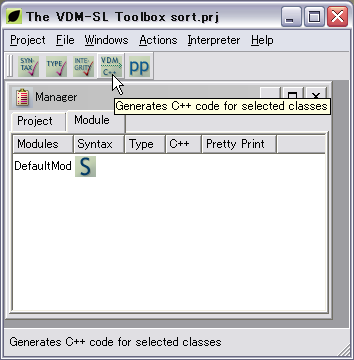
\includegraphics{cgsl1}}
\caption{Code Generating the Sort Example}\label{fig:cg}
\end{center}
\end{figure}
#else
\begin{figure}[tbh]
\begin{center}
\mbox{}
\resizebox{9cm}{!}{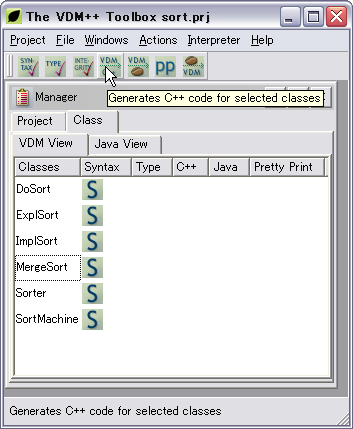
\includegraphics{cgpp1}}
\caption{Code Generating the Sort Example}\label{fig:cg}
\end{center}
\end{figure}
#endif //VDMSL

Code is generated for each \ifthenelse{\boolean{VDMsl}}{module - in
  this example only one - }{class} in the specification and the
Toolbox signals this by writing a big {\em \large{C}} as shown in
Figure~\ref{fig:cg2}. A number of C++ files have been created in the
directory, where your project file lies. If no project file exists,
the files will be written in the directory, where the \ToolboxName\ was
started.

When generating code for the sort example, one warning is generated by
\tcg{}, and the {\em Error} window therefore pops up as
shown in Figure~\ref{fig:cg_error}.

#ifdef VDMSL
\begin{figure}[tbh]
\begin{center}
\mbox{}
\resizebox{9.2cm}{!}{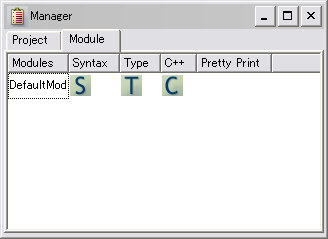
\includegraphics{cgsl2}}
\caption{Code Generating the Sort Example}\label{fig:cg2}
\end{center}
\end{figure}
#else
\begin{figure}[tbh]
\begin{center}
\mbox{}
\resizebox{9.2cm}{!}{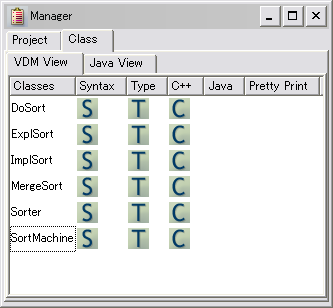
\includegraphics{cgpp2}}
\caption{Code Generating the Sort Example}\label{fig:cg2}
\end{center}
\end{figure}
#endif //VDMSL


#ifdef VDMSL
\begin{figure}[tbh]
\begin{center}
\mbox{}
\resizebox{9.2cm}{!}{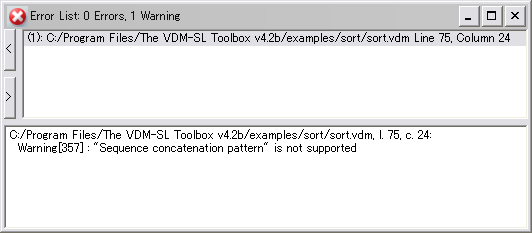
\includegraphics{cgsl3}}
\caption{A Warning Generated by the Code Generator}\label{fig:cg_error}
\end{center}
\end{figure}
#else
\begin{figure}[tbh]
\begin{center}
\mbox{}
\resizebox{9.2cm}{!}{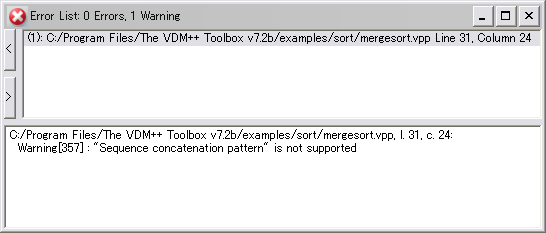
\includegraphics{cgpp3}}
\caption{A Warning Generated by the Code Generator}\label{fig:cg_error}
\end{center}
\end{figure}
#endif //VDMSL


This warning states that the sequence concatenation pattern is not
supported by \tcg{}. This means, that \tcg\ cannot generate executable
C++ code for this construct.  The generated code will be compilable,
but executing the branch containing the unsupported construct will
cause a run-time error. A detailed list of unsupported constructs is
given in Section~\ref{sec:unsupported}.

The user of \tcg\ can choose to generate code containing position
information of run-time errors.  When the {\em Output position
  information} option is chosen, run-time error messages will
tell you the position (file name, line and column number) in the \VDM\ 
specification which causes the run-time error. This feature can be
  set in the option menu, as shown in Figure~\ref{fig:option}.
#ifdef VDMPP
Another option available is the \textit{Check pre and post conditions}
option. This generates code which checks operation
and function pre conditions, and function post conditions. It is also
shown in Figure~\ref{fig:option}.
#endif VDMPP

\begin{figure}[tbh]
\begin{center}
\mbox{}
#ifdef VDMPP
\resizebox{9cm}{!}{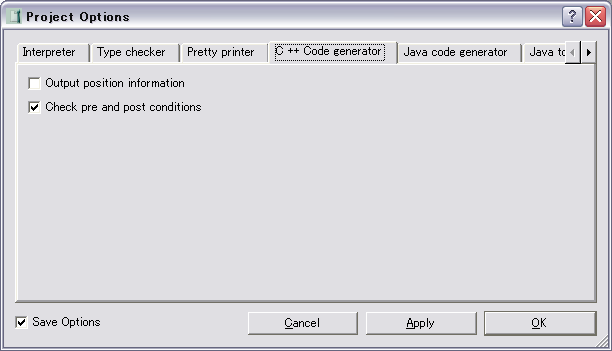
\includegraphics{cgpp4}}
\caption{C++ Code Generator Options}\label{fig:option}
#endif VDMPP
#ifdef VDMSL
\resizebox{9cm}{!}{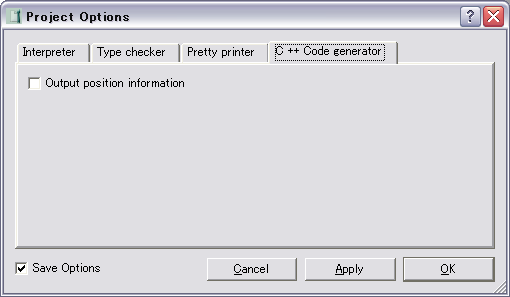
\includegraphics{cgsl4}}
\caption{Option for Generating Position Information in Run-time Errors}\label{fig:option}
#endif VDMSL
\end{center}
\end{figure}
  
For the sort example, the execution of the \texttt{MergeSort} function will,
as described above, result in a run-time error.  Without setting the described 
option, the execution of the corresponding C++ code
will result in the following error message:
\begin{quote}
\begin{verbatim}
The construct is not supported: Sequence concatenation pattern
\end{verbatim}
\end{quote}
On the other hand, when setting the option, the following error message will appear:
#ifdef VDMSL
\begin{quote}
\begin{verbatim}
Last recorded position:
In: sort.vdm. At line: 43 column: 18
The construct is not supported: Sequence concatenation pattern
\end{verbatim}
\end{quote}
#else
\begin{quote}
\begin{verbatim}
Last recorded position:
In: MergeSort. At line: 31 column: 18
The construct is not supported: Sequence concatenation pattern
\end{verbatim}
\end{quote}
#endif

\subsection{Using the Command Line Interface}\label{commandline}

\Tcg\ can of course also be invoked when the \ToolboxName\ is run from
the command line. This will be described briefly in the following.

The \ToolboxName\ is started from the command line with the command {\tt
  \vdmde}\index{vdmde!starting}. The -c option is used in order to
generate code:

#ifdef VDMPP
\begin{quote}
\begin{verbatim}
vppde -c [-r] [-P] specfile, ...
\end{verbatim}
\end{quote}
#else
\begin{quote}
\begin{verbatim}
vdmde -c [-r] specfile, ...
\end{verbatim}
\end{quote}
#endif

In order to code generate the sort example, the following command is
executed in the 
#ifdef VDMSL
\path+vdmhome/examples/sort+ directory:
#endif VDMSL
#ifdef VDMPP
\path+vpphome/examples/sort+ directory:
#endif VDMPP

#ifdef VDMPP
\begin{quote}
\begin{verbatim}
vppde -c *.vpp
\end{verbatim}
\end{quote}
#else
\begin{quote}
\begin{verbatim}
vdmde -c sort.vdm
\end{verbatim}
\end{quote}
#endif

The specification will be parsed first. If no syntax errors are
detected, the specification will be type checked for possible
well-formedness. Finally, if no type errors are detected, the
specification will be translated into a number of C++ files.
Corresponding to the graphical interface, the user can set the {\em
  Output position information} option ({\tt -r}) in order to generate
code with run-time position 
#ifdef VDMPP
information, and the \textit{Check pre and
post conditions} option (\texttt{-P}) to generate run-time checks of
pre and post conditions. 
#else
information.
#endif //VDMPP


\subsection{Generated C++ Files}\label{sec:cppfiles}

Let us now go one step further and look at the files generated by the code generator.

For each 
\ifthenelse{\boolean{VDMsl}}{module}{\VDM\ class}, 
four files are generated:
#ifdef VDMSL
\begin{itemize}
\item {$<$ModuleName$>$.h}\mbox{}
\item {$<$ModuleName$>$.cc}\mbox{}
\item {$<$ModuleName$>$\_anonym.h}
\item {$<$ModuleName$>$\_anonym.cc}
\end{itemize}

The \path+<ModuleName>.h+ file contains C++ function declarations corresponding to
all the functions and operations defined in the specific VDM module. 
Moreover it contains the class definitions corresponding to the composite types defined in the module.

The \path+<ModuleName>.cc+ file contains the implementation of the
functions and operations defined in the specific VDM module. In addition, for
every class generated for a record type, the implementation of its
member functions is found here.

The purpose of the \path+<ModuleName>_anonym.h+ and
\path+<ModuleName>_anonym.cc+ files is to declare and implement
all the anonymous types that appear in the specific module.

The \cg{} supports both code generation of structured and code
generation of flat \VDM\ specifications (see \langmancite). However, a
flat specification is transformed into a default module named {\tt
  DefaultMod}. This module exports all \VDM\ cconstructs (except the
module state).


#else

\begin{itemize}
\item \path+<ClassName>.h+
\item \path+<ClassName>.cc+
\item \path+<ClassName>_anonym.h+
\item \path+<ClassName>_anonym.cc+
\end{itemize}

The \path+<ClassName>.h+ file contains the definition of the C++ class
corresponding to the \VDM\ class. Moreover it contains the class
definitions corresponding to the composite types defined in the \VDM\ 
class.

The \path+<ClassName>.cc+ file contains the implementation of the
functions and operations defined in the \VDM\ class. Moreover, for
every class generated for a record type, the implementation of its
member functions is found here.

The purpose of the \path+<ClassName>_anonym.h+ and 
\path+<ClassName>_anonym.cc+ files is to declare and implement all the
anonymous types. Anonymous types are those that are not given a name
  in the \VDM\ specification.

%When a class \path+M+ for example declares a type {\tt A =
%  set of int}, the \verb+M_anonym.h+ file will contain the declaration
%of a type \verb+type_iS+ and the \path+M.h+ file will contain a
%corresponding C++ \path+typedef+, as explained in the last section.
#endif //VDMSL

#ifdef VDMPP
Apart from these files, two more files are generated:
\begin{itemize}
\item \texttt{CGBase.h}
\item \texttt{CGBase.cc}
\end{itemize}

These files contain part of the implementation of the object reference
type. This is described in Section~\ref{sec:classes}.

%These files contains a class definition of {\em CGBase} which is super
%class to all non-derived classes. The {\em CGBase} class is part of
%modelling object reference of all instances of all the classes in the
%VDM++ specification that is generated. The {\em CGBase} class is
%described in Section~\ref{sec:classes}.
%
%The code corresponding to each \VDM{} class is divided into a header
%and an implementation file. Both files will be named with the class
%name. The suffix for the header file will be '.h', whereas the suffix
%for the implementation file will '.cc' on Unix platforms and '.cpp' on
%Windows platforms. The suffix of the implementation file can be
%customised by setting the environment variable {\bf
%VDMCGEXT}\footnote{On the Windows 95 platform this can be set in the
%\texttt{autoexec.bat} file, and on the Windows NT platform this can be
%set in the \texttt{Registry}}.

#endif //VDMPP

The code corresponding to each \VDM{} 
\ifthenelse{\boolean{VDMsl}}{module}{class}
is divided into a header
and an implementation file. Both files will be named with the 
\ifthenelse{\boolean{VDMsl}}{module}{class}
name. The suffix for the header file will be '\texttt{.h}', whereas the suffix
for the implementation file will '\texttt{.cc}' on Unix platforms and
'\texttt{.cpp}' on 
Windows platforms. The suffix of the implementation file can be
customised by setting the environment variable {\bf
VDMCGEXT}\footnote{On the Windows 2000/XP/Vista platform this can be
set in the \texttt{Registry}}.  

\section{Interfacing the Generated Code}\label{interfacing}

We have now reached the point, where a number of C++ files have been
generated from a \VDM\ specification. 
You are now in the position to write an interface to these C++ files in order to compile, link
and run an application.


To be able to write an interface to the generated code, you
must have some basic knowledge about the generated code. This
includes, first of all, the strategy used when generating code for
\VDM\ constructs, especially \VDM\ types.  In the following, we will 
give a short introduction to this topic. For more information the
reader is referred to Section~\ref{sec:relation}.

#ifdef VDMPP
\subsection{Code Generating VDM++ Types - The Basics}\label{basics}
#else
\subsection{Code Generating VDM-SL Types - The Basics}\label{basics}
#endif//VDMPP
This section gives a short introduction to the way \VDM\ types are
code generated.

Let us start by giving an example of generated C++ code.  The
signature of the function \path+IsOrdered+, 

#ifdef VDMPP
\begin{quote}
\begin{verbatim}
IsOrdered: seq of int -> bool
\end{verbatim}
\end{quote}
#else
\begin{quote}
\begin{verbatim}
IsOrdered: seq of real -> bool
\end{verbatim}
\end{quote}
#endif

\ifthenelse{\boolean{VDMsl}}{defined in module \path+DefaultMod+}{defined in class \path+ExplSort+, }
is for example code generated as follows:

#ifdef VDMPP
\begin{quote}
\begin{verbatim}
class type_iL : public SEQ<Int>{
...
};

Bool vdm_ExplSort::vdm_IsOrdered(const type_iL &vdm_l) {
...
};
\end{verbatim} 
\end{quote}
#else
\begin{quote}
\begin{verbatim}
class type_rL : public SEQ<Real>{
...
};

Bool vdm_DefaultMod_IsOrdered(const type_rL &vdm_DefaultMod_l){
...
};
\end{verbatim} 
\end{quote}
#endif

In order to understand this code, it is necessary to have some
knowledge about the strategy used to generate code for VDM types, as
well as the used name conventions.

The data type handling of \tcg{} is based upon the \MCL{}. The current
version of this library (\path+libvdm.a+) is described in
\libmancite.

\begin{itemize}

\item {\em Basic Data Types}

The basic data types are mapped to the
  corresponding VDM C++ library classes, \path+Bool+, \path+Int+, {\tt
    Real}, \path+Char+ and \path+Token+.

\item {\em Quote Types}

  
  The quote types are mapped into the corresponding VDM C++ library
  class {\tt Quote}.

\item {\em Set, Sequence and Map Types}
  
  To handle the compound types \path+set+, \path+sequence+ and \path+map+, templates are
  introduced. These templates are also defined in the VDM C++ library. As an
  example let us show how the VDM type \verb+seq of int+ is code generated:
\begin{quote}
\begin{verbatim}
class type_iL : public SEQ<Int>{
...
};
\end{verbatim}
\end{quote}

  The VDM \path+seq+ type is mapped into a class that inherits from the
  template \path+SEQ+ class. In case of \verb+seq of int+, the argument
  of the template class is \path+Int+, the C++ class representing the
  basic VDM type \path+int+. The name of the new class is made up in the following way:

\begin{quote}
\verb+type+ : signals an anonymous type\\
\verb+i+: signals int\\
\verb+L+: signals sequence\\
\end{quote}

\item {\em Composite/Record Types}
  
  Each composite type is mapped into a class that is a subclass of the
  VDM C++ library \path+Record+ class. For example, the following composite
  type defined \ifthenelse{\boolean{VDMsl}}{in module \path+M+}{in class \path+M+}
\begin{quote}
\begin{verbatim}
A:: r : real
    i : int
\end{verbatim}
\end{quote}
will be code generated as:
\begin{quote}
\begin{verbatim}
class TYPE_M_A : public Record{
...
};
\end{verbatim}
\end{quote}

\item {\em Tuple Types}

The strategy for handling tuples is very similar to that of composite types.
Each tuple type is mapped into a class that is a subclass of the 
VDM C++ library \path+Tuple+ class. For example, the following tuple:
\begin{quote}
\begin{verbatim}
int * real
\end{verbatim}
\end{quote}
will be code generated as:
\begin{quote}
\begin{verbatim}
class type_ir2P : public Tuple{
...
};
\end{verbatim}
\end{quote}

The name of the new class is made up in the following way:

\begin{quote}
\verb+type+ : signals an anonymous type\\
\verb+i+: signals int\\
\verb+r+: signals real\\
\verb+2P+: signals tuple with size two.\\
\end{quote}

\item {\em Union Types}

The union type is mapped into the VDM C++ library \path+Generic+ class. 

\item {\em Optional Types}

The optional type is mapped into the VDM
  C++ library \path+Generic+ class.

#ifdef VDMPP

\item {\em Object Reference Types}

For each VDM++ class a corresponding C++ class is generated. For a VDM++
class {\em SortMachine} a corresponding C++ class {\em
  vdm\_SortMachine} will be generated. 

An object reference of an instance of class is mapped into a class
\path+type_ref_<ClassName>+.

The object reference type is described in detail in
Section~\ref{sec:classes}. 
#endif

\end{itemize}


The composite type example has already given you an idea about the way,
type names are generated. 

Types that are not given a name in the specification (anonymous types)
are prefixed with \path+type+ written with small letters. Type names
however are prefixed with \path+TYPE+ written with capital letters.  In the
record example we have seen one example of a type name, namely {\tt
  TYPE\_M\_A}. The other \VDM\ types can of course also be named and
the name scheme used is the same as for records.

A generated type name is prefixed with \path+TYPE+. Then it is followed
by the \ifthenelse{\boolean{VDMsl}}{module name}{class name}, where the type is defined, and finally the chosen
VDM name is concatenated.  

Take a look at the following \VDM\ specification and the name conventions
used when generating the defined types:

#ifdef VDMPP
\begin{quote}
\begin{verbatim}
class M
types
  A = int;
  B = int * real;
  C = seq of int;
end M
\end{verbatim}
\end{quote}
#else
\begin{quote}
\begin{verbatim}
module M
exports all
definitions
types
  A = int;
  B = int * real;
  C = seq of int;
end M
\end{verbatim}
\end{quote}
#endif

The three defined types above will be given the names \verb+TYPE_M_A+,
\verb+TYPE_M_B+ and \verb+TYPE_M_C+. The scope of these type names is
limited to the \ifthenelse{\boolean{VDMpp}}{class}{module}\ \path+M+. The
definition of these names is therefore placed in file {\em
  M.h}. 

\begin{verbatim}
 #define TYPE_M_A Int 
 #define TYPE_M_B type_ir2P 
 #define TYPE_M_C type_iL
\end{verbatim}


However, the specification also contains two anonymous types {\tt
  int * real} and \verb+seq of int+. These types can potentially be
used in any \ifthenelse{\boolean{VDMpp}}{class}{module}, and therefore the
name and definition of the corresponding C++ type should be 
declared and defined globally\footnote{The strategy is to define unique names
  for structurally equal types.  This strategy is used in order to
  solve the fact that C++ is based on type name equivalence, whereas
  VDM++ is based on structural equivalence. }. This is done in the
{\em anonym} files: 
#ifdef VDMSL
\path+<ModuleName>_anonym.{cc,h}+
#else
\path+<ClassName>_anonym.{h,cc}+
#endif //VDMSL


In addition to the information given about the way types are
code generated, it should be mentioned how function or operation names
are generated: A function or operation name \path+f+ in a
\ifthenelse{\boolean{VDMsl}}{module}{class} M in a VDM specification
will be given the name:
#ifdef VDMSL
\path+vdm_M_f+.
#else
\path+vdm_M::vdm_f+.
#endif //VDMSL

You should now have an idea about \tcg{}'s overall strategy when
generating code for VDM specifications. More detailed information is
given in Section~\ref{sec:relation} and should be studied carefully
before using \tcg\ professionally.

\subsection{Files to be Implemented by the User}

We have now given some basic information about \tcg\ and the code
generated files. This section describes the work the user must do in
order to interface with the generated code.

Let us start by giving you an overview of all the C++ files involved
when running the C++ code for a \VDM\ specification. These files can
be split up into code generated C++ files and handcoded C++ files.
Figure~\ref{fig:cppfiles} shows the code generated files to the left
and the handcoded files to the right. Moreover, the involved files can
be split up into C++ files per \VDM\ 
\ifthenelse{\boolean{VDMsl}}{module}{class} and C++ files per \VDM\ 
specification.

\begin{figure}[tbh]
\begin{center}
\begin{picture}(400,300)(0,0)
\put(0,0){\framebox(150,70)[c]{%
  \parbox{4.5cm}{
#ifdef VDMPP
  \texttt{<Classname>.h}
  \texttt{<Classname>.cc}
  \texttt{<Classname>\_anonym.h}
  \texttt{<Classname>\_anonym.cc}
#endif VDMPP
#ifdef VDMSL
  \texttt{<Modulename>.h}
  \texttt{<Modulename>.cc}
  \texttt{<Modulename>\_anonym.h}
  \texttt{<Modulename>\_anonym.cc}
#endif VDMSL
  }
}}

\put(250,0){\framebox(150,70)[c]{
  \parbox{5cm}{
#ifdef VDMPP
  \texttt{<Classname>\_userdef.h}
  \texttt{<Classname>\_userimpl.cc}
#endif VDMPP
#ifdef VDMSL
  \texttt{external\_<Modulename>.h}
  \texttt{external\_<Modulename>.cc}
#endif VDMSL
  }
}}

#ifdef VDMPP
\put(0,230){\framebox(150,70)[c]{
  \parbox{4.5cm}{
    \texttt{CGBase.h}
    \texttt{CGBase.cc}
  }
}}
#endif VDMPP

\put(250,230){\framebox(150,70)[c]{
  \parbox{4.5cm}{
    Main program
  }
}}

\put(125,115){\framebox(150,70)[c]{
  \parbox{4.5cm}{
    \VDM\ Specification/ Project
  }
}}

\put(125,115){\vector(-1,-1){44}}
\put(275,115){\vector(1,-1){44}}
#ifdef VDMPP
\put(125,185){\vector(-1,1){44}}
#endif VDMPP
\put(275,185){\vector(1,1){44}}

\put(200,35){\makebox(0,0){\parbox{2.4cm}{%
  \raggedright C++ files per \VDM\ 
    \ifthenelse{\boolean{VDMsl}}{module}{class}
  }
}
}

\put(200,265){\makebox(0,0){\parbox{2.4cm}{%
\raggedright C++ files per \VDM\ project}
}}

\put(75,150){\makebox(0,0){\parbox{2.4cm}{%
\raggedright Code generated C++ files}}}

\put(325,150){\makebox(0,0){\parbox{2.4cm}{%
\raggedright Hand coded C++ files}}}

\end{picture}


\caption{C++ Files per \VDM\ Project}\label{fig:cppfiles}
\end{center}
\end{figure}

Section~\ref{sec:cppfiles} has already described the code generated C++ files. We will now decribe the handcoded files.

To interface with the generated code the user has to perform the following tasks:

\begin{enumerate}
\item For each \ifthenelse{\boolean{VDMsl}}{module}{class}
      define offsets for record tags.
\item Implement implicit functions/operations and
  specification statements contained in the \VDM\ specification.
\item Write a main program.
\item Optionally, substitute parts of the generated C++ code with
handwritten code. 
\item Compile, link and run the application.

\end{enumerate}

In the following we will describe these tasks one by one for the sort
example.

\subsubsection{Definition of Offsets for Record Tags}

A composite type (record type) consists in the \VDM\ specification of
a string (the tag) and a sequence of field selections for each field 
in the record type:

\begin{quote}
\begin{verbatim}
RecTag ::
  fieldsel1 : nat
  fieldsel2 : bool
\end{verbatim}
\end{quote}

In the VDM C++ Library the record tag string {\em ``RecTag''} is
modelled with a unique integer. However, it is important for this
strategy that all record types within one specification have their own
unique tag number. For each 
\ifthenelse{\boolean{VDMpp}}{class}{module}\ \tcg\ will number the
record tags sequentially from an offset basis.  The offset should be
defined by the user, and it is the responsibility of the user that the
offsets defined for each \ifthenelse{\boolean{VDMpp}}{class}{module}\ 
ensures that the tags are unique.

The definition of the offset should be written in a file called
#ifdef VDMSL
\path+<ModuleName>_userdef.h+
#else
\path+<ClassName>_userdef.h+
#endif //VDMSL
%\ifthenelse{\boolean{VDMsl}}{\path+<ModuleName>_userdef.h+}
%{\path+<ClassName>_userdef.h+}. 
The offset should be defined with a
define directive. The name of the tag offset should be
#ifdef VDMSL
\path+TAG_<ModuleName>+.
#else
\path+TAG_<ClassName>+.
#endif //VDMSL
%\ifthenelse{\boolean{VDMpp}}{\path+TAG_<ClassName>+}{\path+TAG_<ModuleName>+}.

#ifdef VDMPP
For the sort example this implies, that the user has to implement 6
files, one for each class. The \verb+MergeSort_userdef.h+ file, for
example, could possibly contain the following definition.

\begin{verbatim}
 #define TAG_MergeSort 100
\end{verbatim}

#else 

For the sort example this
implies, that the user has to implement one file, namely \path+DefaultMod_userdef.h+. This file could possibly contain the
following definition.

\begin{verbatim}
 #define TAG_DefaultMod 100
\end{verbatim}

#endif

\subsubsection{Implementing Implicit Functions/Operations and Specification
  Statements}\label{implicit}

For every \ifthenelse{\boolean{VDMsl}}{module}{class} which contains
an implicit function a
#ifdef VDMSL
\path+<ModuleName>_userimpl.cc+
#else
\path+<ClassName>_userimpl.cc+
#endif //VDMSL
%\ifthenelse{\boolean{VDMsl}}{\path+<ModuleName>_userimpl.cc+}{\path+<ClassName>_userimpl.cc+}
file containing the function definition has to be written.

#ifdef VDMPP

The sort example contains one implicit function in the \path+ImplSort+
class, namely \path+ImplSorter+. This function must be implemented in
the file \path+ImplSort_userimpl.cc+ in order to interface the generated C++ code.
The function has to be written in such a way that it
matches its member function declaration which can be found
in class \path+vdm_ImplSort+, defined in file \path+ImplSort.h+:

\begin{quote}
\begin{verbatim}
virtual type_iL vdm_ImplSorter(const type_iL &);
\end{verbatim}
\end{quote}

The function \path+ImplSorter+ in class \path+ImplSort+ is given the name
\path+vdm_ImplSort::vdm_ImplSorter+ and has the following declaration:

\begin{quote}
\begin{verbatim}
type_iL vdm_ImplSort::vdm_ImplSorter(const type_iL& l) {
...
}
\end{verbatim}
\end{quote}

One possible implementation of this function 
is shown in Appendix \ref{sec:implsort}.
#endif VDMPP

#ifdef VDMSL

The sort example contains one implicit function, namely \path+ImplSort+. This function must be implemented in
the file \verb+DefaultMod_userimpl.cc+ in order to interface the generated C++ code.
The function has to be written in such a way, that it
matches the generated C++ function declaration. 
This can be found
in file \path+DefaultMod.h+:

\begin{quote}
\begin{verbatim}
type_rL vdm_DefaultMod_ImplSort(const type_rL &);
\end{verbatim}
\end{quote}

The function \path+ImplSort+ in module \path+DefaultMod+ is given the name
{\tt vdm\_De\-fault\-Mod\_Impl\-Sort}.

One possible implementation of this function 
is listed in Appendix \ifthenelse{\boolean{VDMpp}}{\ref{sec:implsort}}{\ref{sec:userimpl}}.

#endif VDMSL

Thus, the user has to write a C++ function definition for
the operation and add it to the
#ifdef VDMSL
\path+<ModuleName>_userimpl.cc+
#else
\path+<ClassName>_userimpl.cc+
#endif //VDMSL
file of the \ifthenelse{\boolean{VDMsl}}{module}{class} which contains the operation.


The code generator generates an include directive for each
specification statement it meets. Thus, for each specification
statement the user has to implement a corresponding file with the
name: 
#ifdef VDMSL
\path+vdm_<ModuleName>_<OperationName>-<No>.cc+, 
#endif VDMSL
#ifdef VDMPP
\path+vdm_<ClassName>_<OperationName>-<No>.cc+, 
#endif VDMPP
where
\path+<OperationName>+ is the name of the operation in which the
specification statement appears, and \path+<No>+ is a sequential
numbering of the specification statements that appear in the specific
operation. 



\subsubsection{Implementing the Main Program}
We have now implemented the files necessary to compile, link and run
the code, except for the main program. 

Let us therefore write a main program for 
the sort example.

#ifdef VDMPP 
First of all, we will start by specifying the  main program in \VDM{}.

\begin{quote}
\begin{verbatim}
01   Main: () ==> ()
02   Main () ==
03     let arr1 = [3,5,2,23,1,42,98,31],
04         arr2 = [3,1,2] in
05  
06     ( dcl smach : SortMachine := new SortMachine(),
07           res : seq of int = [];
08       def dos : Sorter := new DoSort() in
09       res = smach.SetAndSort(dos,arr1);
10       def expls : Sorter := new ExplSort() in
11       res = smach.SetAndSort(expls,arr2);
12       def imps  : Sorter := new ImplSort() in
13       ( res = smach.SetAndSort(imps,arr2)
14         imps.Post_ImplSorter(arr2,res)
15       )
16      def mergs : Sorter := new MergeSort() in
17       smach.SetSort(mergs);
18      res = smach.GoSorting(arr2);
19     )
\end{verbatim}
\end{quote}

We will now implement a C++ main program with the same functionality
as in the above specified \VDM\ method. The main program is
implemented in the file \path+sort_pp.cc+ and the complete program is
shown in appendix \ref{sec:main}.

The C++ file, containing the main program, should start by including all the necessary header files.
These include one header file per \VDM\ class, the header of the
\MCL{}, called \path+metaiv.h+, and the standard library class
\path+<fstream>+ (in order to generate output).

Let us now, step by step, translate the above listed VDM specification
to C++.
%\footnote{One could also code generate the listed \VDM\ 
%  specification and then write a main program calling the generated
%  \path+vdm_Main+ function. However, this would not be very helpful in
%  learning something about the way to interface with the generated
%  code. Moreover, it would not be possible to generate some output.}
%
Line \path+03+ and \path+04+ specify two integer lists.
Translated to C++, one will get the following code:
\begin{quote}
\begin{verbatim}
type_iL arr1, arr2;
arr1.ImpAppend ((Int)3);
arr1.ImpAppend ((Int)5);
...
arr2.ImpAppend ((Int)3).ImpAppend ((Int)1).ImpAppend ((Int)2);
\end{verbatim}
\end{quote}

Line \path+06+ declares an object reference \path+smach+ to an instance
of the class \path+SortMachine+. 

The following line implements this in C++:
\begin{quote}
\begin{verbatim}
type_ref_SortMachine smach (ObjectRef (new vdm_SortMachine ()));
\end{verbatim}
\end{quote}

Line \path+07+ declares a variable \path+res+ of type \verb+seq of int+,
which will later be used to contain the sorted integer sequences. The
C++ code for this is just:

\begin{quote}
\begin{verbatim}
type_iL res;
\end{verbatim}
\end{quote}

Let us now show how to call a specific sorting method.  

As can be seen from the \VDM\ specification and the generated C++
code, the class \path+SortMachine+ has an object reference to the
abstract class \path+Sorter+ as an instance variable.  The subclasses
of \path+Sorter+ implement the different sorting algorithms.  The
method \path+SetAndSort+ of the \path+SortMachine+ class takes two
parameters: An instance of a subclass of \path+Sorter+ and a sequence
of integers. The method sets the mentioned instance variable to refer
to the specified subclass and thereby to a specific sorting algorithm,
and it afterwards calls the \path+Sort+ method of this class with the
integer sequence as parameter. The result will be a sorted integer
sequence.

Line \path+08+ declares an object reference \path+dos+ to an instance of
the class \path+DoSort+, and line \path+08+ calls the \path+SetAndSort+
method of the \path+SortMachine+ class with the declared object
reference \path+dos+ and the integer sequence \path+arr1+ as arguments.
The result is assigned to \path+res+.  

All code generated \VDM\ types have an \path+ascii+ method which
returns a string containing an ASCII representation of the respective
VDM value.  This method is being used here to print relevant log
messages to standard output during execution. A reference to the {\tt
  SortMachine} class can be obtained by calling the
\verb+ObjGet_vdm_SortMachine+ function defined in the code generated
class {\tt CGBase}

\begin{quote}
\begin{verbatim}
cout << "Evaluating DoSort(" << arr1.ascii () << "):\n";
type_ref_Sorter dos (ObjectRef (new vdm_DoSort ()));
res = ObjGet_vdm_SortMachine(smach)->
        vdm_SetAndSort (dos, arr1);
cout << res.ascii() << "\n\n";
\end{verbatim}  
\end{quote}

In order to sort \path+arr2+ with the sorting algorithm defined in
class \path+ExplSort+, the following code can be written analogously:
\begin{quote}
\begin{verbatim}
cout << "Evaluating ExplSort(" << arr2.ascii () << "):\n";
type_ref_Sorter expls (ObjectRef(new vdm_ExplSort ()));
res = ObjGet_vdm_SortMachine(smach)->
        vdm_SetAndSort (expls, arr2);
cout << res.ascii() << "\n\n";
\end{verbatim}
\end{quote}

In order to sort \path+arr2+ with the sorting algorithm implemented  in
class \path+ImplSort+, the following code can be written:
\begin{quote}
\begin{verbatim}
cout << "Evaluating ImplSort(" << arr2.ascii () << "):\n";
type_ref_Sorter imps (ObjectRef(new vdm_ImplSort ()));
res = ObjGet_vdm_SortMachine(smach)->
        vdm_SetAndSort (imps, arr2);
cout << res.ascii() << "\n\n";
\end{verbatim}
\end{quote}
Note, that the interface to the code is independent of having
implicit or explicit functions/operations.

One could also imagine that one wants to call the post condition function
for \path+ImplSort+. \Tcg\ has generated a function called 
\path+vdm_post_ImplSorter+ in class \path+vdm_ImplSort+ for it. This
function can be called in the ususal way. 
\begin{quote}
\begin{verbatim}
cout << "Evaluating post condition for ImplSort:\n";
Bool p = ObjGet_vdm_ImplSort(imps)->
           vdm_post_ImplSorter (arr2, res);
cout << "post_ImplSort(" << arr2.ascii () << "," <<
  res.ascii () <<  "):\n" << p.ascii () << "\n\n";
\end{verbatim}
\end{quote}

Instead of calling the \path+SetAndSort+ method of the {\tt
  SortMachine} class, one can choose to first set the desired sorting
algoritm by calling \path+SetSort+ and afterwards to call the {\tt
  GoSorting} method, as shown in line \path+16+ to \path+18+.  We choose
here the \path+MergeSort+ algorithm, well-knowing that the resulting
C++ code will imply a run-time error.  The resulting code is shown in
the following:

\begin{quote}
\begin{verbatim}
type_ref_Sorter mergs (ObjectRef(new vdm_MergeSort ()));
ObjGet_vdm_SortMachine(smach)->vdm_SetSort (mergs);

cout << "Evaluating MergeSort(" << arr2.ascii () << "):\n";
res = ObjGet_vdm_SortMachine(smach)->vdm_GoSorting(arr2);
cout << res.ascii() << "\n\n";
\end{verbatim}  
\end{quote}


%?? The \MCL{} is implemented in a way such that compound types can
%?? contain elements of any VDM type (\path+Generic+). This means that an
%?? object of any VDM C++ class can automatically be casted to a {\tt
%??   Generic}. For example, the \VDM{} type \path+seq of nat+ is
%?? translated into a \path+Sequence+ in the generated code.
%??

The described main program is implemented in the file named 
\path+sort_pp.cc+ and it is listed in Appendix \ref{sec:main}. 

#endif VDMPP

#ifdef VDMSL

First of all, we will start by specifying the  main program in \VDM{}.

\begin{quote}
\begin{verbatim}
01    Main: () ==> ()
02    Main() ==
03    let l = [0, -12, 45] in
04    ( dcl res : seq of real,
05          b  : bool;
06      res := DoSort(l);
07      res := ExplSort(l);
08      res := ImplSort(l);
09      b  := post_ImplSort(l, res);
10      b  := inv_PosReal(hd l);
11      b  := inv_PosReal(hd res);
12      res := MergeSort(l))
\end{verbatim}
\end{quote}

We will now implement a C++ main program with the same functionality
as in the above specified \VDM\ method. The main program is
implemented in the file \path+sort_ex.cc+ and the complete program is
shown in appendix \ref{sec:main}.

The C++ file, containing the main program, should start by including all the necessary header files.
These include one header file per \VDM\ module, the header of the
\MCL{}, called \path+metaiv.h+, and the standard library class
\path+<fstream>+ (in order to generate output).

\begin{quote}
\begin{verbatim}
// Initialize values in DefaultMod
init_DefaultMod();
\end{verbatim}
\end{quote}

Let us now, step by step, translate the above listed VDM specification
to C++.
%\footnote{One could also code generate the listed \VDM\ specification
%  and then write a main program calling the generated \path+vdm_Main+
%  function. However, this would not be very helpful in learning
%  something about the way to interface with the generated code.
%  Moreover, it would not be possible to generate some output.}.
%
Line \path+03+ specifies a list of reals.
Translated to C++, one will get the following code:
\begin{quote}
\begin{verbatim}
type_rL l;
l.ImpAppend(Int(0));
l.ImpAppend(Int(-12));
l.ImpAppend(Int(45));
\end{verbatim}
\end{quote}

Line \path+04+ declares a variable \path+res+ of type \texttt{seq of real},
which will later be used to contain the sorted sequence. Line \path+05+
declares a variable of type \path+bool+. The C++ code for this is just:
\begin{quote}
\begin{verbatim}
type_rL res;
Bool b;
\end{verbatim}
\end{quote}

Let us now show how to call a specific sorting method.  

Line \path+06+ calls the \path+DoSort+ function with the declared list of reals as argument.
The result will be a sorted sequence.

All code generated \VDM\ types have an \path+ascii+ method which
returns a string containing an ASCII representation of the respective VDM value.
This method is being used here to print relevant log messages to \path+cout+
(standard output) during execution.
\begin{quote}
\begin{verbatim}
cout << "Evaluating DoSort(" << l.ascii() << "):\n";
res = vdm_DefaultMod_DoSort(l);
cout << res.ascii() << "\n\n";
\end{verbatim}  
\end{quote}

In order to sort \path+l+ with the function \path+ExplSort+ or \path+ImplSort+, the following code can be written analogously:
\begin{quote}
\begin{verbatim}
cout << "Evaluating ExplSort(" << l.ascii() << "):\n";
res = vdm_DefaultMod_ExplSort(l);
cout << res.ascii() << "\n\n";
\end{verbatim}
\end{quote}

\begin{quote}
\begin{verbatim}
cout << "Evaluating ImplSort(" << l.ascii() << "):\n";
res = vdm_DefaultMod_ImplSort(l);
cout << res.ascii() << "\n\n";
\end{verbatim}
\end{quote}
Note, that the interface to the code is independent of having
implicit or explicit functions/operations.

One could also imagine, that one wants to call the post condition function
for \path+ImplSort+. \Tcg\ has generated a function called 
{\tt vdm\-\_De\-fault\-Mod\-\_post\-\_Impl\-Sort} for it. This
function can be called in the ususal way. 
\begin{quote}
\begin{verbatim}
cout << "Evaluating the post condition of ImplSort. \n"
     << "post_ImplSort(" << l.ascii() << ", "
     << res.ascii() << "):\n";
b = vdm_DefaultMod_post_ImplSort(l, res);
cout << b.ascii() << "\n\n";
\end{verbatim}
\end{quote}
  
  As can be seen from the \VDM\ specification and the generated C++
  code, \tcg\ has generated an invariant function for the invariant
  defined for the type \path+PosReal+. This function is called {\tt
    vdm\_DefaultMod\_inv\_PosReal} and it can be called in the ususal
  way:

\begin{quote}
\begin{verbatim}
cout << "Evaluation the invariant of PosReal. \n"
     << "inv_PosReal(" << l.Hd().ascii() << "):\n";
b = vdm_DefaultMod_inv_PosReal(l.Hd());
cout << b.ascii() << "\n\n";

cout << "Evaluation the invariant of PosReal. \n"
     << "inv_PosReal(" << res.Hd().ascii() << "):\n";
b = vdm_DefaultMod_inv_PosReal(res.Hd());
cout << b.ascii() << "\n\n";
\end{verbatim}
\end{quote}

Finally, we can choose to call the \path+MergeSort+ function (line \path+12+), well knowing, that this will imply a run-time error.

\begin{quote}
\begin{verbatim}
cout << "Evaluating MergeSort(" << l.ascii() << "):\n";
res = vdm_DefaultMod_MergeSort(l);
cout << res.ascii() << "\n\n";
\end{verbatim}  
\end{quote}


%??? 
%??? The \MCL{} is implemented in a way such that compound types can
%??? contain elements of any VDM type (\path+Generic+). This means that an
%??? object of any VDM C++ class can automatically be casted to a {\tt
%???   Generic}. For example, the \VDM{} type \path+seq of nat+ is
%??? translated into a \path+Sequence+ in the generated code.
%??? 

The described main program is implemented in the file named {\tt
  sort\_ex.cc} and it is listed in appendix \ref{sec:main}. 

#endif VDMSL

\subsubsection{Substituting Parts of the Generated C++ code}\label{substituting}

Finally, we should say some words about the possibilities of substituting
generated C++ code with handwritten code. This can mainly be useful in two situations:

\begin{itemize}
\item The user wants to implement code for constructs that are not
  supported by \tcg{}.
\item The user wants to implement some existing components more
  efficiently.
\end{itemize}

For the sort example, one could imagine that the user wants to
implement a handcoded version of the \ifthenelse{\boolean{VDMsl}}{{\tt
    MergeSort}}{\path+MergeSorter+} function, as it contains a
construct not supported by \tcg{}. The user then has to substitute the
code generated function 
#ifdef VDMSL
\path+vdm_DefaultMod_MergeSort+
#else
\path+vdm_MergeSort::vdm_MergeSorter+
#endif //VDMSL
with a handcoded version. In order to do so, a new
function has to be written. This must have the same declaration header
as the code generated version found in
#ifdef VDMSL
\path+DefaultMod.cc+:
#else
\path+MergeSort.cc+:
#endif //VDMSL


#ifdef VDMPP
\begin{quote}
\begin{verbatim}
type_rL vdm_MergeSort::vdm_MergeSorter(const type_rL &vdm_l) {
...
}
\end{verbatim}
\end{quote}
#else
\begin{quote}
\begin{verbatim}
type_rL vdm_DefaultMod_MergeSort(const type_rL 
                                       &vdm_DefaultMod_l) {
...
}
\end{verbatim}
\end{quote}
#endif

In order to substitute a code generated function with a handwritten
function, the function has to be
implemented in a file named 
#ifdef VDMSL
\path+DefaultMod_userimpl.cc+
#else
\path+MergeSort_userimpl.cc+
#endif //VDMSL
and the
following two defines have to be added to the
#ifdef VDMSL
\path+DefaultMod_userdef.h+
#else
\path+MergeSort_userdef.h+
#endif //VDMSL
file:


#ifdef VDMPP
\begin{quote}
\begin{verbatim}
 #define DEF_MergeSort_USERIMPL    
   // a user defined file is now included.Note: For classes
   // containing implicit functions/operations, an user
   // implemented file is a presumption and this line should be
   // obmitted.
 #define DEF_MergeSort_MergeSorter 
   //  the MergeSorter function in class MergeSort is handcoded 
\end{verbatim}
\end{quote}

#else
\begin{quote}
\begin{verbatim}
 #define DEF_DefaultMod_MergeSort 
 //  the MergeSort function in module DefaultMod is hand coded
\end{verbatim}
\end{quote}

For modules that do not contain an implicit function or operation
definition, a \path+<ModuleName>_userimpl.cc+ is optional. If the file
is created the user
has to add another line to the \path+<ModuleName>_userdef.h+ file
in order to specify that a \path+<ModuleName>_userimpl.cc+ file now
exists:
\begin{quote}
\begin{verbatim}
 #define DEF_DefaultMod_USERIMPL
\end{verbatim}
\end{quote}
#endif

In this way, you can substitute specific functions generated by \tcg\ with
handwritten functions.

\subsection{Compiling, Linking and Running the C++ code}
After the user has handwritten the above described files, he is now
in a position to compile, link and run the C++ code.

C++ code generated by this version of the \cg{} must be compiled using
one of the following supported compilers:

\begin{itemize}
\item Microsoft Windows 2000/XP/Vista and Microsoft Visual C++ 2005 SP1
\item Mac OS X 10.4 or higher
\item Linux GNU gcc 3, 4 and Kernel 2.4, 2.6
\item Solaris 10
\end{itemize}

In order to create an executable application,
the code must be linked to the following libraries:

\begin{itemize}
\item \path+libCG.a+: Code generator auxiliary functions. This library
  is released with the \cg{} and is described in Appendix
  \ref{sec:libCG}.
\item \path+libvdm.a+: The \MCL{}. This library is released with the
  \cg{} and is described in \libmancite.
\item \path+libm.a+: The math library corresponding to the compiler.
\end{itemize}


#ifdef VDMPP

The \path+Makefile+ used in the implementation of the sort
example is listed in appendix \ref{sec:make}. To compile the main
program \path+sort_pp+, you must type \path+make+ \path+sort_pp+.

% Note that all the classes in the example are code generated in advance.

#endif VDMPP

#ifdef VDMSL

The \path+Makefile+ used in the implementation of the sort
example is listed in Appendix \ref{sec:make}. To compile the main
program \path+sort_ex+, you must type \path+make sort_ex+.

#endif VDMSL

#ifdef VDMPP
You can now run the main program \path+sort_pp+.
Its output is listed below.
Note that a run-time error has occurred during execution
of \path+MergeSort+. This is caused by the fact that we have tried to
execute an unsupported construct.  The position information which has
been included in the generated code, leads to the origin of the
error in the underlying specification.

\begin{quote}
\begin{verbatim}
$  sort_pp
Evaluating DoSort([ 3,5,2,23,1,42,98,31 ]):
[ 1,2,3,5,23,31,42,98 ]

Evaluating ExplSort([ 3,1,2 ]):
[ 1,2,3 ]

Evaluating ImplSort([ 3,1,2 ]):
[ 1,2,3 ]

Evaluating post condition for ImplSort:
post_ImplSort([ 3,1,2 ],[ 1,2,3 ]):
true

Evaluating MergeSort([ 3,1,2 ]):
Last recorded position:
In: MergeSort. At line: 26 column: 18
The construct is not supported: Sequence concatenation pattern
$
\end{verbatim}
\end{quote}

#else
You can now run the main program \path+sort_ex+.
Its output is listed below.
Note that a run-time error has occurred during execution
of \path+MergeSort+. This is caused by the fact that we have tried to
execute an unsupported construct.  The position information which has
been included in the generated code, leads to the origin of the
error in the underlying specification.

\begin{quote}
\begin{verbatim}
$ sort_ex
Evaluating DoSort([ 0,-12,45 ]):
[ -12,0,45 ]

Evaluating ExplSort([ 0,-12,45 ]):
[ -12,0,45 ]

Evaluating ImplSort([ 0,-12,45 ]):
[ -12,0,45 ]

Evaluating the post condition of ImplSort. 
post_ImplSort([ 0,-12,45 ], [ -12,0,45 ]):
true

Evaluation the invariant of PosReal. 
inv_PosReal(0):
true

Evaluation the invariant of PosReal. 
inv_PosReal(-12):
false

Evaluating MergeSort([ 0, -12, 45 ]):
Last recorded position:
In: sort.vdm. At line: 43 column: 18
The construct is not supported: Sequence concatenation pattern
$
\end{verbatim}
\end{quote}
#endif

\section{Unsupported Constructs}\label{sec:unsupported}

In this version of \tcg\ the following \VDM\ constructs are
not supported:

\begin{itemize}

%% Is not part of the language manual any longer!
%\item The Real-time part of \VDM{}. 
\item Expressions:

  \begin{itemize}
  \item Lambda.
  \item Compose,  iterate and equality for functions.
  \item Function type instantiation expression. However, the code
    generator supports function type instantiation expression in
    combination with apply expression, as in the following example:

\begin{quote}
\begin{verbatim}
Test:() -> set of int
Test() ==
  ElemToSet[int](-1);

ElemToSet[@elem]: @elem +> set of @elem
ElemToSet(e) ==
  {e}
\end{verbatim}
\end{quote}

#ifdef VDMPP
\item The concurrency part of \VDM{}, that is the
 {\tt \#act}, {\tt \#fin} {\tt \#active}, {\tt \#waiting} and
  {\tt \#req} expressions.

#endif VDMPP
  \end{itemize}

\item Statements: 

  \begin{itemize}
#ifdef VDMSL
  \item `{\sf using}' in call statement.
#endif VDMSL
  \item Always, exit, trap and recursive trap statements.
#ifdef VDMPP
  \item Start and start list statements.
#endif VDMPP
  \end{itemize}

\item Type binds (see \langmancite) in:

  \begin{itemize}
  \item Let-be-st expression/statements.
  \item Sequence, set and map comprehension expressions.
  \item Iota and quantified expressions.
  \end{itemize}

As an example the following expression is supported by \tcg :


\begin{quote}
\begin{verbatim}
let x in set numbers in x
\end{verbatim}
\end{quote}

whereas the following is not (caused by the type bind \verb+n: nat+):

\begin{quote}
\begin{verbatim}
let x: nat in x
\end{verbatim}
\end{quote}

\item Patterns:

  \begin{itemize}
  \item Set union pattern.
  \item Sequence concatenation pattern.
  \end{itemize}

#ifdef VDMSL
\item Local Function Definitions.

\item Higher order function definitions.
  
\item Function Values. 

\item Parameterized modules.
#endif VDMSL

#ifdef VDMPP
\item Threads
\item Synchronization definitions
#endif VDMPP
\end{itemize}

\Tcg\ is able to generate compilable code for
specifications including these constructs, but the execution of the
code will result in a run-time error if a branch containing an
unsupported construct is executed. Consider the following function
definition:

\begin{quote}
\begin{verbatim}
f: nat -> nat
f(x) ==
  if x <> 2 then
    x
  else
    iota x : nat & x ** 2 = 4
\end{verbatim}
\end{quote}

In this case code for \path+f+ can be generated and compiled.  The
compiled C++ code corresponding to \path+f+ will result in a run-time
error if \path+f+ is applied with the value 2, as type binds in iota
expression are not supported.

Note that \Tcg\ will give a warning whenever an
unsupported construct is encountered.

%\section{Trouble Shooting\label{sec:trouble}}
%- not all classes are syntax checked
%- VDMSL: init function is not called.
%- Tag offset is not used properly.
%

%\section{Advanced Example\label{sec:advanced}}

%!!!!!!!!!!!!!!!!!to be written? !!!!!!!!!!!!!!!!!!!

\section{Code Generating VDM Specifications - The Details}\label{sec:relation}

This section will give you a detailed description of the way \VDM\ 
constructs are code generated, including
\ifthenelse{\boolean{VDMsl}}{modules}{classes}, types, functions,
operations, \ifthenelse{\boolean{VDMsl}}{states}{instance variables},
values, expressions and statements.

This description should be studied intensively if you want to use \tcg\ 
professionally. 

Note: This section focuses on the different \VDM\ constructs and their
mapping to C++ code, NOT on the overall structure of the generated C++
files. The reader is referred to Section~\ref{sec:cppfiles} and
Section~\ref{interfacing} for a description of the overall structure.


#ifdef VDMPP
\subsection{Code Generating Classes}\label{sec:classes}
#endif //VDMSL


#ifdef VDMPP

For each VDM++ class a corresponding C++ class is generated. The inheritance
structure of the VDM++ classes corresponds exactly to the inheritance
structure of the generated C++ classes. However, the generated classes
are tightly coupled to the \MCL, as it is the case for all the generated types
in \tcg. In order to fully understand how the type system works in
the generated code you should read the documentation of this
library \libmancite.  However, we will give a small introduction to
the \MCL\ below.

\subsubsection{Object References in the \MCL}

The \MCL\ is structured with two superclasses: {\em Common} and {\em
  MetaivVal}. For every \VDM\ type a corresponding C++ class exists
which is a subclass to {\em Common}, and correspondingly for every
kind of value in \VDM\ a corresponding C++ class exists which is
a subclass to {\em MetaivVal}. Thus, the \MCL\ is structured in a type
and a value system, as it is illustrated in Figure~\ref{fig:mcl}.

\begin{figure}[tbh]
\begin{center}
\begin{picture}(400,140)(0,0)
\put(0,0){\framebox(40,40){Map}}
\put(60,0){\framebox(40,40){\parbox{1.5cm}{\begin{center}Object\- Ref\end{center}}}}
\put(120,20){\makebox(0,0){$\cdots$}}
\put(140,0){\framebox(40,40){Int}}

\put(200,0){\framebox(40,40){\parbox{1.5cm}{\begin{center}Map- Val\end{center}}}}
\put(260,0){\framebox(40,40){\parbox{1.5cm}{\begin{center}vdm\-Base\end{center}}}}
\put(320,20){\makebox(0,0){$\cdots$}}
\put(340,0){\framebox(40,40){IntVal}}

\put(70,80){\framebox(60,60){Common}}
\put(40,40){\line(1,1){40}}
\put(95,40){\line(0,1){40}}
\put(155,40){\line(-1,1){40}}
\put(129,90){\makebox(0,0)[r]{p}}
\put(130,90){\vector(1,0){140}}

\put(270,80){\framebox(60,60){MetaivVal}}
\put(240,40){\line(1,1){40}}
\put(295,40){\line(0,1){40}}
\put(355,40){\line(-1,1){40}}


\end{picture}
\caption{The overall Structure of \MCL\ }\label{fig:mcl}
\end{center}
\end{figure}


When an object of a class, say \path+Int+, is created then an
object of {\em IntVal} is created automatically too, which contains the integer value.
In addition the pointer \path+p+ from the \path+Int+ object will be set
to point to that \path+IntVal+ object.

Let us now have look at how the \VDM\ type ``object reference'' is
reflected in the \MCL. As for all other types, the \MCL\ provides two
classes: in the value part system the class {\tt vdmBase} and in the
type part system class \path+ObjectRef+. When creating an instance of
an \path+ObjectRef+, the constructor takes a pointer to an object of
the corresponding value part side as input, that is an object of class
{\tt vdmBase}. The declaration of one of the typically used
constructors of the \path+ObjectRef+ class is listed below:

\begin{verbatim}
class ObjectRef : public Common {
 public:
   ...
   ObjectRef(vdmBase* = NULL);
   ...
}
\end{verbatim}


\subsubsection{The Inheritance Structure of the Generated Code of Classes}

\Tcg\ uses the object reference support of the \MCL\ in
the following way. All the C++ classes corresponding to VDM++ classes inherit
from the \path+vdmBase+ class. In addition, for every class in the
\VDM\ specification a corresponding class is generated that represents
the object reference of exactly this \VDM\ class. This C++ class
inherits from the \path+ObjectRef+ class.

The inheritance structure of the generated C++ class of the sorting
example and the \MCL\ is shown in Figure~\ref{fig:sortppmcl}.

\begin{figure}[H]
\begin{center}
\begin{picture}(400,440)(0,0)
\put(58,294){\makebox(0,0){$\cdots$}}
\put(90,270){\framebox(48,48){\parbox{1.5cm}{\begin{center}Object\- Ref\end{center}}}}
\put(170,294){\makebox(0,0){$\cdots$}}


\put(230,294){\makebox(0,0){$\cdots$}}
\put(262,270){\framebox(48,48){\parbox{1.5cm}{\begin{center}vdm\-Base\end{center}}}}
\put(342,294){\makebox(0,0){$\cdots$}}

\put(90,358){\framebox(48,48){Common}}
\put(114,318){\line(0,1){40}}
\put(137,364){\makebox(0,0)[r]{p}}
\put(138,364){\vector(1,0){124}}


\put(262,358){\framebox(48,48){
  \parbox{1.7cm}{
  \begin{center}
  Metaiv Val
  \end{center}
}}}
\put(286,318){\line(0,1){40}}

\put(0,90){\framebox(48,48){\parbox{1.7cm}{%
  \begin{center}\small
  type\_\-ref\_\-Merge\-Sort
  \end{center}
}}}

\put(60,90){\framebox(48,48){\parbox{1.7cm}{%
  \begin{center}\small
  type\_\-ref\_\-Expl\-Sort
  \end{center}
}}}

\put(120,90){\framebox(48,48){\parbox{1.7cm}{%
 \begin{center}\small
   type\_\-ref\_\-Impl\-Sort
  \end{center}
}}}

\put(180,90){\framebox(48,48){\parbox{1.7cm}{%
  \begin{center}\small
  type\_\-ref\_\-DoSort
  \end{center}
}}}


\put(30,180){\framebox(48,48){\parbox{1.7cm}{%
  \begin{center}
  type\_\-ref\_ Sort\-Machine
  \end{center}
}}}

\put(90,180){\framebox(48,48){\parbox{1.7cm}{%
  \begin{center}
  type\_\-ref\_ Sorter
  \end{center}
}}}
\put(114,228){\line(0,1){42}}
\put(54,228){\line(1,1){42}}



\put(48,138){\line(1,1){42}}
\put(180,138){\line(-1,1){42}}
\put(104,138){\line(0,1){42}}
\put(122,138){\line(0,1){42}}


\put(262,90){\framebox(48,48){\parbox{1.7cm}{%
  \begin{center}\small
  vdm\_ Sorter
  \end{center}
}}}

\put(322,90){\framebox(48,48){\parbox{1.7cm}{%
  \begin{center}\small
  vdm\_ Sort\- Machine
  \end{center}
}}}


\put(352,0){\framebox(48,48){\parbox{1.7cm}{%
  \begin{center}\small
  vdm\_ \-Merge\-Sort
  \end{center}
}}}

\put(292,0){\framebox(48,48){\parbox{1.7cm}{%
  \begin{center}\small
  vdm\_ \-Expl\-Sort
  \end{center}
}}}

\put(232,0){\framebox(48,48){\parbox{1.7cm}{%
  \begin{center}\small
  vdm\_ \-Impl\-Sort
  \end{center}
}}}

\put(172,0){\framebox(48,48){\parbox{1.7cm}{%
  \begin{center}\small
  vdm\_ \-DoSort
  \end{center}
}}}

\put(352,48){\line(-1,1){42}}
\put(220,48){\line(1,1){42}}
\put(275,48){\line(0,1){42}}
\put(295,48){\line(0,1){42}}


\put(262,180){\framebox(48,48){\parbox{1.7cm}{%
  \begin{center}\small
  CGBase
  \end{center}
}}}

\put(286,228){\line(0,1){42}}

\put(286,138){\line(0,1){42}}
\put(346,138){\line(-1,1){42}}

\end{picture}
\caption{The inheritance structure of the C++ classes of the sorting
  example and the \MCL\ }\label{fig:sortppmcl}
\end{center}
\end{figure}

In the type system part specialised object reference classes are
generated \path+type_ref_<Classname>+ for each VDM++ class.
Consider the declaration the class \path+type_ref_DoSort+:

\begin{verbatim}
class type_ref_DoSort : public virtual type_ref_Sorter {
public:
  type_ref_DoSort() : ObjectRef() {}
  type_ref_DoSort(const Generic &c) : ObjectRef(c) {}
  type_ref_DoSort(vdmBase * p) : ObjectRef(p) {}
  const char * GetTypeName() const { return "type_ref_DoSort"; }
} ;
\end{verbatim}

The class contains a constructor that takes a pointer to the {\tt
  vdmBase} class. Constructing an object reference to an object of
class \path+ExplSort+ can be done in the following way:

\begin{verbatim}
  type_ref_DoSort ds (new vdm_DoSort());
\end{verbatim}


As it can be seen from Figure~\ref{fig:sortppmcl},  the generated C++
classes do not inherit directly from the {\em
  vdmBase}, but through the class {\em CGBase}. This class is also
generated by \tcg.

The \path+CGBase+ class is declared and defined in the files {\em
  CGBase.cc} and {\em CGBase.h}. Apart from the class definition the
{\em CGBase} files also consist of definitions of some extern
functions. Altogether, this code provides functions that make it
possible to extract the value part (that is the actual C++ object
reference) of the object reference type.

For the {\em Sorting} example consider an extract of the {\em CGBase.h}
file:

\begin{verbatim}
class CGBase : public vdmBase {
private:
  ....
public:
  virtual vdm_DoSort * Get_vdm_DoSort() { return 0; }
  ....
  virtual vdm_Sorter * Get_vdm_Sorter() { return 0; }
};
vdm_DoSort * ObjGet_vdm_DoSort(const ObjectRef &obj);
...
vdm_Sorter * ObjGet_vdm_Sorter(const ObjectRef &obj);
enum  {
  VDM_DoSort,
  ...
  VDM_Sorter
};
\end{verbatim}

For each VDM++ class a global function is generated: 
\path+ObjGet_vdm_<ClassName>.+ The function takes an {\em ObjectRef}
and returns a pointer to the corresponding object of the C++ class.
Furthermore, a unique tag is defined for each class description.

An example of constructing an object reference and applying the functions
within the class \path+DoSort+ is given below:

\begin{verbatim}
   type_iL somelist;
   type_ref_DoSort ds (new vdm_DoSort);
   ObjGet_vdm_Sorter(ds)->vdm_Sort(somelist);
\end{verbatim}

As the implementation of the \MCL\ is based on reference
counters, it will delete the pointer to the instance of class 
\path+vdm_A+ when no existing objects of class \path+ObjectRef+ refer to it.
To illustrate this, consider the following example:

\begin{quote}
\begin{verbatim}
{ 
  type_ref_DoSort ds(new vdm_DoSort);
  {
    type_ref_DoSort tmp(new vdm_DoSort);
    ds = tmp; // at this point the first vdm_DoSort
              // pointer will be deleted.
  }
} // The second vdm_DoSort pointer will be deleted when 
  // this scope is closed.
\end{verbatim}
\end{quote}

You should {\bf never} directly declare a pointer to a vdm class and
instantiate this to an {\em ObjectRef}. This can go wrong
because the \MCL\ is based on reference counters, and will delete the
objects when there is pointer (at least from the point of view of the
\MCL) that points at the object reference.

\begin{quote}
\begin{verbatim}
{ 
  vdm_DoSort * ds_p = new vdm_DoSort();       // Never do this
  {                                           // Never do this
    type_ref_DoSort tmp(ds_p);                // Never do this
    ...                                       // Never do this
  } // Now the ds_p will be deleted.          // Never do this
  ...                                         // Never do this
} 
\end{verbatim}
\end{quote}


\subsubsection{The Structure of a Generated Class}

The generated C++ classes contain:

\begin{itemize}
\item C++ functions that implement \VDM\ functions and operations.
\item Some auxiliary functions for object reference gymnastics.
\item Constructors/destructors of the class.
\end{itemize}
The access modifiers in the class follow those specified in the \VDM\
class, with the exception of type definitions, for which it is not
meaningful to give an access modifier. Thus for example a function
which is public at the VDM++ level will be code generated as a public
member of the corresponding C++ class, and so on.

Consider the declaration of the C++ \path+vdm_DoSort+ class:
\begin{verbatim}
class vdm_DoSort : public virtual vdm_Sorter {

  friend class init_DoSort ;

public:
  vdm_DoSort * Get_vdm_DoSort () { return this;  }
  ObjectRef Self () { return ObjectRef(Get_vdm_DoSort());  }
  int vdm_GetId () { return VDM_DoSort;  }
  vdm_DoSort ();
  virtual ~vdm_DoSort () {}

private:
  virtual type_iL vdm_DoSorting (const type_iL &);
  virtual type_iL vdm_InsertSorted (const Int &, const type_iL &);

public:
  virtual type_iL vdm_Sort (const type_iL &);
};
\end{verbatim}

The class consists of the VDM++ functions \path+vdm_DoSorting+, 
\path+vdm_InsertSorted+ and \path+vdm_Sort+. 

The auxiliary functions are:
\begin{itemize}
\item \texttt{Get\_vdm\_DoSort}: returns the reference pointer to the object self.
\item \texttt{Get\_vdm\_Self}: returns the object reference pointer to the
  object self.
\item \texttt{vdm\_GetId}: returns the unique tag of the class.
\end{itemize}
#endif 

%#ifdef VDMSL
%\subsection{Code Generating Modules}\label{sec:classes}

%For each module


%#endif //VDMSL


\subsection{Code Generating Types}\label{types}

In Section~\ref{basics} we have already given a short introduction to the
way \VDM\ types are mapped into C++ code. 

Here we will give a more detailed description of this topic.

Section~\ref{motivation} gives a motivation for the strategy used when
code generating \VDM\ types.  Section~\ref{mapping} then describes the
mapping of each \VDM\ type into C++ code.
Section~\ref{nameconventions} summarizes the used name conventions for
types.

\subsubsection{Motivation}\label{motivation}

The type scheme of \tcg\ can be split into two parts:
\begin{itemize}
\item The type scheme used in function headers of the generated C++ code.
\item The type scheme used in the rest of the generated C++ code.
\end{itemize}
The type scheme used in function headers uses C++ types that have
been code generated. The type scheme used in the rest of
the generated code uses the fixed implementation of each \VDM\ data
type found in the \MCL{}.
The VDM C++ library (\path+libvdm.a+) is
described in \libmancite.

Let us imagine we have a VDM function with a \path+seq of char+ as
input parameter.  Then the corresponding C++ function will take a
parameter of type \path+type_cL+ as input. The type \path+type_cL+ is a
code generated type, where \path+c+ resembles the VDM type \path+char+,
and \path+L+ resembles the VDM type \path+seq+. The function
implementation however uses only the type \path+Sequence+ found in the \MCL{} instead of
the type \path+type_cL+.

The code generated types obviously improve the generated C++ code.
They offer the possibility of catching more type errors at compilation
time, and they are more informative for the user.

With the introduction of new types a new problem arise: We have to
ensure, that a \verb+seq of char+ in
\ifthenelse{\boolean{VDMsl}}{module}{class} \path+A+ is the same type
as a \verb+seq of char+ in \ifthenelse{\boolean{VDMsl}}{module}{class}
\path+B+.

#ifdef VDMPP
\begin{quote}
\begin{verbatim}
class A
types
  C = seq of char
end A

class B
types
  D = seq of char
end B
\end{verbatim}
\end{quote}
#else
\begin{quote}
\begin{verbatim}
module A
exports all
definitions
types
  C = seq of char
end A

module B
exports all
definitions
types
  D = seq of char
end B
\end{verbatim}
\end{quote}
#endif
In \VDM\ the types \verb+A`C+ and \verb+B`D+ are equivalent. This is
however not the case in C++, because C++ uses name
equivalence except for the basic data types.

The generated code has to ensure two things:

\begin{itemize}
\item An anonymous \VDM\ type may only be code generated once in order to
  ensure type correctness in the generated code.
  
\item The generated type name should be readable and understandable.
\end{itemize}

#ifdef VDMPP
The first problem is solved by generating \path+<Class+ \path+Name>_anonym+%PathForcedLineBreak
files.  The \path+<Class+ \path+Name>_anonym.h+%PathForcedLineBreak
file contains type declarations for all types that are potentially
declared by other classes (anonymous types) as well. The
\path+<ClassName>_anonym.cc+ contains the implementation of these
types.  Moreover, it contains macro defintions for them.

Note, that types which are not anonymous, i.e. composite types and
type names, are not declared in the {\tt $<$ClassName$>$\_anonym.h} file,
but instead in the \path+<ClassNa+ \path+me>.h+%PathForcedLineBreak
file.
#else
The first problem is solved by generating \path{<ModuleName>anonym}
files.  The \path{<Module} \path{Name>_anonym.h} file contains type
declarations for all types that are potentially also declared in other
modules (anonymous types). The \path+<ModuleName>_anonym.cc+ contains the
implementation of these types.  
Moreover, it contains macro defintions for them. 

Note, that types which are not anonymous, i.e. composite types and
type names, are not declared in the \path+<ModuleName>_anonym.h+ file,
but instead in the \path+<Module+ \path+Name>.h+%PathForcedLineBreak
file.  

#endif

Let us show you the anonymous header file generated for \ifthenelse{\boolean{VDMsl}}{module}{class} A in the
above listed example.

\path+A_anonym.h+ looks like:
\begin{quote}
\begin{alltt}
class type\_cL;

\#define TYPE\_A\_D type_cL

\#ifndef TAG\_type\_cL
\#define TAG\_type\_cL (TAG\_A + 1)
\#endif

\#ifndef DECL\_type\_cL
\#define DECL\_type\_cL 1
class type\_cL : public SEQ<Char> {
...
}
\#endif
\end{alltt}
\end{quote}



The first {\tt \#define} statement defines a macro for type \path+D+ in module \path+A+.
It will be replaced with type \path+type_cL+. The \path+TAG_type_cL+
ensures a unique tag for the type \path+type_cL+ in the generated
code. The two {\tt \#ifndef} statements ensure that the 
\path+TAG_type_cL+ and the \path+type_cL+ are only defined once, either
in the file \path+A_anonym.h+ or in the file \path+B_anonym.h+.

The second problem is solved by the chosen name conventions for
generated C++ types. The strategy for generating type names is to
unfold types into what we could call a canonical form and then give
the canonical form a name based on the type names and type constructors
involved. The next two subsections will give you more information
about the used notation.

#ifdef VDMPP
\subsubsection{Mapping VDM++ Types to C++}\label{mapping}
#else
\subsubsection{Mapping VDM-SL Types to C++}\label{mapping}
#endif //VDMPP
This section describes how VDM types are mapped into C++ types.

\begin{itemize}

\item {\em The Boolean Type}

  
  The VDM \path+bool+ type is mapped to the VDM C++ library class {\tt
    Bool} and it is abbreviated with the character \path+b+.  


\item {\em The Numeric Types}

The VDM {\tt
    nat}, \path+nat1+ and \path+int+ types are all mapped to the VDM C++
  library class \path+Int+ and they are abbreviated with the character \path+i+.
  The VDM \path+real+ and \path+rat+ types are mapped to the VDM C++
  library class \path+Real+ and they are abbreviated with the character \path+r+.

\item {\em The Character Type}

  The VDM type \path+char+ is mapped to the VDM C++ library class {\tt
    Char} and it is abbreviated with the character \path+c+.

\item {\em The Quote Type}


The VDM Quote type is mapped to the VDM C++ library class \path+Quote+
and it is abbreviated with the character \path+Q+.  As for all
types, a unique tag has to be ensured for quotes.
In the following we will show how the quote \verb+<Hello>+ is code
generated.

The following code will be added in the file {\tt $<$ClassName$>$\_anonym.h}:

\begin{quote}
\begin{alltt}
extern const Quote quote_Hello;
\#define TYPE\_A\_C Quote
\#ifndef TAG\_quote\_Hello
\#define TAG\_quote\_Hello (TAG\_A + 1)
\#endif
\end{alltt}
\end{quote}

The following code will be added in the file {\tt $<$Clasname$>$\_anonym.cc}:

\begin{quote}
\begin{alltt}
\# if !DEF_quote_Hello && DECL_quote_Hello
\# define DEF_quote_Hello 1
const Quote quote_Hello("Hello");
\#endif
\end{alltt}
\end{quote}

The declared quote value may now be referenced as \path+quote_Hello+ in
the C++ code.

\item {\em The Token Type}

The token type is implemented using the C++ class \path+Record+.
However, the tag of token records is always equal to \path+TOKEN+,
which is a macro declared in the file \path+cg_aux.h+ (see Appendix
\ref{sec:libCG}), and the number of fields in token records is always
equal to 1. The \VDM{} value {\tt mk\_token(<HELLO>)} can e.g.\ be
constructed in the following way:

\begin{quote}
\begin{verbatim}
Record token(TOKEN, 1); 
token.SetField(1, Quote("HELLO"));
\end{verbatim}
\end{quote}

\item {\em The Sequence Type}

To handle the compound types \path+set+, \path+sequence+ and \path+map+,
templates are introduced. These templates are also defined in the VDM
C++ library and they are based on the C++ classes \path+Set+, \path+Sequence+ and
 \path+Map+ in the C++ VDM library.

The \path+seq+ type is abbreviated with the character \path+L+.
As an
  example let us show how the VDM type \verb+seq of int+ is code generated:
\begin{quote}
\begin{verbatim}
class type_iL : public SEQ<Int> {
public:
  type_iL() : SEQ<Int>() {}
  type_iL(const SEQ<Int> &c) : SEQ<Int>(c) {}
  type_iL(const Generic &c) : SEQ<Int>(c) {}
  const char * GetTypeName() const { return "type_iL"; }
} ;
\end{verbatim}
\end{quote}
The VDM \path+seq+ type is mapped into a class that inherits from the
template \path+SEQ+ class. In case of \verb+seq of int+, the argument
of the template class is \path+Int+, the C++ class representing the
basic VDM type \path+int+. The name of the new class is made in the
following way:

\begin{quote}
\verb+type+ : signals an anonymous type\\
\verb+i+: signals int\\
\verb+L+: signals sequence\\
\end{quote}

Note also that several constructors for the \path+type_iL+ class have
been generated together with a \path+GetTypeName+ function.

\item {\em The Set Type}
  
  The VDM \path+set+ type is handled in the same way as the VDM {\tt
    seq} type. The template class \path+SET+ is used rather than {\tt
    SEQ} and the type is abbreviated with the character \path+S+.

\item {\em The Map Type} 

The VDM \path+map+ type is handled in the same
  way as the VDM \path+seq+ type. The template class \path+MAP+ is used
  rather than \path+SEQ+ and the \path+Map+ template class takes two
  arguments rather than one. The \path+map+ type is abbreviated with
  the character \path+M+.



\item {\em The Composite/Record Type}
  
  Each composite type is mapped into a class that is a subclass of the
  VDM C++ library \path+Record+ class. For example, the following composite
  type defined in a class \path+M+

\begin{quote}
\begin{verbatim}
A:: c : real
    k : int
\end{verbatim}
\end{quote}

will be code generated as:
\begin{quote}
\begin{verbatim}
class TYPE_M_A : public Record {
public:
  TYPE_M_A() : Record(TAG_TYPE_M_A, 2) {}
  TYPE_M_A(const Generic &c) : Record(c) {}
  const char * GetTypeName() const { return "TYPE_M_A"; }
  TYPE_M_A &Init(Real p1, Int p2);

  Real get_c() const;
  void set_c(const Real &p);
  Int get_k() const;
  void set_k(const Int &p);
} ;
\end{verbatim}
\end{quote}

As you can see, a record named \path+A+ in a
\ifthenelse{\boolean{VDMsl}}{module}{class} \path+M+ will be given the
name: \verb+TYPE_M_A+.

Several member functions have been added to the generated C++ class definition:

\begin{itemize}
\item
Two constructors have been added.
\item
The function \path+GetTypeName+ has been added.
\item An initialisation function \path+Init+ has been added. This
  function initialises the record fields to the corresponding values
  of the input parameters and returns a reference to the object.
\item For each field in the record, two member functions have been
  added in order to get and set its value.  The names of these
  functions match the names of the corresponding VDM record field
  selectors.  If a field selector is missing, the position of the
  element in the record will be used instead, e.g. \verb+get_1+.
\end{itemize}

The implementation of the \path+Init+ function and the {\tt set/get}
functions can be found in the implementation file of the class, where
the record type has been defined.  For the above defined record type,
the following code can be found in the file \path+M.cc+:

\begin{quote}
\begin{verbatim}
TYPE_M_A &TYPE_M_A::Init(Real p1, Int p2) {
  SetField(1, p1);
  SetField(2, p2);
  return * this;
}

Real TYPE_M_A::get_c() const { return (Real) GetField(1); }
void TYPE_M_A::set_c(const Real &p) { SetField(1, p); }
Int TYPE_M_A::get_k() const { return (Int) GetField(2); }
void TYPE_M_A::set_k(const Int &p) { SetField(2, p); }

\end{verbatim}
\end{quote}

\item {\em The Tuple/Product Type}

The strategy for handling tuples is very similar to that of composite types.
Each tuple type is mapped into a class that is a subclass of the 
VDM C++ library \path+Tuple+ class. For example, the following tuple:

\begin{quote}
\begin{verbatim}
int * real
\end{verbatim}
\end{quote}

will be code generated as:

\begin{quote}
\begin{verbatim}
class type_ir2P : public Tuple {
public:

  type_ir2P() : Tuple(2) {}
  type_ir2P(const Generic &c) : Tuple(c) {}
  const char * GetTypeName() const { return "type_ir2P"; }
  type_ir2P &Init(Int p1, Real p2);
  Int get_1() const;
  void set_1(const Int &p);
  Real get_2() const;
  void set_2(const Real &p);
} ;
\end{verbatim}
\end{quote}

The name of the new class is made in the following way:

\begin{quote}
\verb+type+ : signals anonymous type\\
\verb+i+: signals int\\
\verb+r+: signals real\\
\verb+2P+: signals tuple with two subtypes/elements\\
\end{quote}

There is however one difference between the code generation of
composite types and tuple types.  The \VDM\ tuple type is an anonymous
type.  Therefore, the C++ type definition is found in the 
\path+<ClassName>_anonym.h+ file, not in the \path+<Classname>.h+ file.
Likewise, the implementation of the member functions is found in the
\path+<Classname>_anonym.cc+, not in the \path+<Classname>.cc+ file.

\item {\em The Union Type}

The union type is mapped into the VDM C++ library \path+Generic+ class. 

\item {\em The Optional Type}
  
  The optional type is mapped into the VDM C++ library \path+Generic+
  class.

Note, \path+nil+ is a special \VDM{} value (not a type).

#ifdef VDMPP

\item {\em The Object Reference Type}

In Section~\ref{sec:classes} it has been described how
two C++ classes are generated for each \VDM\ class.  One of these
represents the class itself and the other one is used for handling a
reference to the \VDM\ class.


Look at the following example:
\begin{quote}
\begin{verbatim}
class M
types
A = seq of N
end M

class N
...
end N
\end{verbatim}
\end{quote}
Class M defines a type \path+A+ that is a reference to an object of
class \path+N+.  When code generating this example, five classes will
be defined: \path+vdm_M+, \path+vdm_N+, \path+type_ref_M+, 
\path+type_ref_N+ and \path+type_1NRL+.
The last one represents the defined type \path+seq of N+.
The name of the new class is made in the following way:

\begin{quote}
\verb+type+ : signals anonymous type\\
\verb+1+: signals numbers of characters in the name of the class\\
\verb+N+: signals class N\\
\verb+R+: signals object reference\\
\verb+L+: signals sequence\\
\end{quote}

Moreover, the following macro will be defined in file \path+M_anonym.h+:
\begin{quote}
\begin{verbatim}
#define TYPE_M_A type_1NRL
\end{verbatim}
\end{quote}


%The \texttt{ObjectRef} constructor must be called with a pointer to an
%object of a code generated \VDM{} class or with a value of type
%\texttt{ObjectRef}. Consider the following VDM++ class:
%
%\begin{quote}
%\begin{verbatim}
%class A
%
%  methods 
%    m() value nat ==
%     return 10
%
%end A
%\end{verbatim}
%\end{quote}
%
%You can create an object reference of class \path+A+ in the
%following way:
%
%\begin{quote}
%\begin{verbatim}
%ObjectRef obj(new vdm_A());
%\end{verbatim}
%\end{quote}
%
%From the \VDM{} specification 
%\begin{quote}
%\begin{verbatim}
%dcl A1 : @A := A!new;
%    A2 : @A := A1;
%\end{verbatim}
%\end{quote}
%
%you can create the C++ object references in the following way:
%\begin{quote}
%\begin{verbatim}
%ObjectRef A1 (new vdm_A);
%ObjectRef A2 (A1);
%\end{verbatim}
%\end{quote}
%
%
%In order to invoke the method \path+m+ in the object reference {\tt
%  obj} the following steps are required:
%
%\begin{quote}
%\begin{verbatim}
%// dcl res : nat := obj!m();
%Int res; 
%vdm_A * p = ObjGet_vdm_A(obj); 
%res = p->vdm_m(); 
%\end{verbatim}
%\end{quote}
%
%The \texttt{ObjGet\_vdm\_A} will return with a null pointer if
%\texttt{obj} is not of type \texttt{vdm\_A}. You can take advantage of
%this like this in the code:
%
%\begin{quote}
%\begin{verbatim}
%vdm_A * p = null;
%if (p=ObjGet_vdm_A (obj))
%  res = p->vdm_m();
%else {
%  cout << "Error: ObjectRef not of type vdm_A" << "\n";
%  ...
%}
%\end{verbatim}
%\end{quote}
%
%If an object reference is not initialised any attempt to extract the
%pointer will result in a run time error.
%
%% If an object reference is not initialised you will get a run time
%% error if you try to extract the
%% 
%% Trying to extract a class pointer from an uninitialised object
%% reference will result in an run time error. 
%% 
%% Trying to extract a class pointer from an uninitialised object
%% reference will result in an run time error. 

%As the implementation of the VDM C++ library is based on reference
%counters, it will delete the pointer to the instance of class 
%\path+vdm_A+ when no existing objects of class \path+ObjectRef+ refer to it.
%To illustrate this, consider the following example:
%
%\begin{quote}
%\begin{verbatim}
%{ 
%  ObjectRef obj(new vdm_A);
%  {
%    ObjectRef tmp(new vdm_A);
%    obj = tmp; // at this point the first vdm_A
%               // pointer will be deleted.
%  }
%} // The second vdm_A pointer will be deleted when 
%  // this scope is closed.
%\end{verbatim}
%\end{quote}
%
%
#endif VDMPP

\end{itemize}

#ifdef VDMSL
\subsubsection{Code Generating VDM-SL Type Names}\label{nameconventions}
#endif VDMSL
#ifdef VDMPP
\subsubsection{Code Generating VDM++ Type Names}\label{nameconventions}
#endif VDMPP

The type system of \VDM\ and C++ differs as C++ uses name equivalence
and \VDM\ uses structural equivalence. In \VDM\
\begin{verbatim}
type                            
  A = seq of int;              
  B = seq of int
\end{verbatim}
type A and B are equivalent because they are
structural equal. However, the corresponding example in C++ is not
equivalent because the name of A and B are different.

\Tcg\ solves this problem by generating equal names for
structural equal types.
Thus, the corresponding generated C++ code is (in essence):

#ifdef VDMSL
\begin{verbatim}
 class type_iL

 class type_iL : public SEQ<Int> {
 public:
   ...
 } ;

 #define TYPE_ModuleName_A type_iL
 #define TYPE_ModuleName_B type_iL
\end{verbatim}
#endif //VDMSL

#ifdef VDMPP
\begin{verbatim}
 class type_iL

 class type_iL : public SEQ<Int> {
 public:
   ...
 } ;

 #define TYPE_ClassName_A type_iL
 #define TYPE_ClassName_B type_iL
\end{verbatim}
#endif //VDMPP

Thus all type name definitions are defined through \#define directives
to a name reflecting the structural content of the type definition.

A generated type name is prefixed with \path+TYPE+ followed
by the \ifthenelse{\boolean{VDMsl}}{module name}{class name}, where
the type is defined and finally the chosen VDM name is concatenated.

All anonymous types, i.e. types that are not given a name in the
\VDM\ specification are prefixed with \path+type+ and a constructed
name that reflects the structure of the type. The type name is based
on an unfolding of the VDM type and the use of a reverse polish
notation. 



%The last subsection described the mapping from \VDM\ types to C++
%code. These \VDM\ types have however not been named (except the
%defined composite type). We will now explain how typenames are code generated.
%
%Types are prefixed with \path+type+ written with small letters. Type
%names however are prefixed with \path+TYPE+ written with big letters.
%In the record example we have seen one example of a type name, namely
%\path+TYPE_M_A+. The other \VDM\ types can of course also be named and
%the used name scheme is the same as for records:
%
%
%Look at the following \VDM\ specification and the name conventions
%used when generating the defined types:
%
%#ifdef VDMPP
%\begin{quote}
%\begin{verbatim}
%class M{
%types
%  A = int;
%  B = int * real;
%  C = seq of int;
%}
%\end{verbatim}
%\end{quote}
%#else
%\begin{quote}
%\begin{verbatim}
%module M
%exports all
%definitions
%types
%  A = int;
%  B = int * real;
%  C = seq of int;
%end M
%\end{verbatim}
%\end{quote}
%#endif
%
%The three defined types above will be given the names \verb+TYPE_M_A+,
%\verb+TYPE_M_B+ and \verb+TYPE_M_C+. The definition of all
%non-composite types implies moreover a macro declaration in
%the \ifthenelse{\boolean{VDMsl}}{\path+<ModuleName>_anonym.h+}{\path+<ClassName>_anonym.h+} file.
%
%The \verb+M_anonym.h+ file will in the just given example contain the following three \path+define+'s:
%
%\begin{quote}
%\begin{verbatim}
%\#define TYPE_M_A Int
%\#define TYPE_M_B type_ir2P
%\#define TYPE_M_C type_iL
%\end{verbatim}
%\end{quote}
%
%This is because non-composite types are global types. A {\tt seq of
%  int} will be a \path+seq of int+, independently of where it is used.
%However a record type \path+A+ in
%\ifthenelse{\boolean{VDMsl}}{module}{class} \path+M+ will not be the
%same type as a record type \path+A+ in
%\ifthenelse{\boolean{VDMsl}}{module}{class} \path+N+, although they
%have the same fields.
%
%
%\subsubsection{Name Conventions for C++ Types\label{nameconventions}}
%
%In order to generate C++ type names that can be understood by humans,
%the typename is created based on an unfolding of the VDM type and the
%use of a reverse polish notation.
%

The table below sketches the naming convention. 
The names of the VDM types and type constructors are in the first
column. In the second row the scheme for generating names
corresponding to the VDM type is listed. In the
second column {\em $<$tp$>$'s} should be replaced by generated type names for
the corresponding VDM type. E.g. the VDM type \verb+map char to int+
is given the name \verb+ciM+ as \verb+char+ translates to \verb+c+,
\verb+int+ translates to \verb+i+ and the map type constructor takes
the two argument types and combines with what we could see as a
reverse polish operator \verb+M+, giving \verb+ciM+. The naming
conventions will be described further in the rest of this note.

\begin{longtable}{|l|l|p{7cm}|} \hline
  VDM            & translation   & examples \\ \hline \hline
\endhead
\hline
\endfoot
\hline
  bool           & \verb+b+      & \verb+b+ \\ \hline
  nat1           & \verb+i+      & \verb+i+ \\ 
  nat            & \verb+i+      & \verb+i+ \\ 
  int            & \verb+i+      & \verb+i+ \\ \hline
  real           & \verb+r+      & \verb+r+ \\ 
  rat            & \verb+r+      & \verb+r+ \\ \hline
  char           & \verb+c+      & \verb+c+ \\ \hline
  quote          & \verb+Q+      & \verb+<Hello>+ translates to \verb+Q+  \\ \hline
  token          & \verb+T+      & \verb+token+ translates to \verb+T+     \\ \hline
  set            & \verb+<tp>S+  & \verb+set of char+ translate to \verb+cS+       \\ \hline
  sequence       & \verb+<tp>L+  & \verb+sequence of real+ translates to \verb+rL+  \\ \hline
  map            & \verb+<tp1><tp2>M+ & \verb+map set of int to char+ translates to \verb+iScM+ \\ \hline
  product        & \verb+<tp1>..<tpn><n>P+ & \verb+int * char * sequence of real+ translates to \verb+icrS3P+ \\ \hline
  composite      & \verb+<length><name>C+ & the composite type \verb+Comp+ translates to \verb+4CompC+. 
                                            Notice that \verb+<length>+ is the number of characters in the name of the composite type. \\ \hline 
  union          & \verb+U+ & \verb+int | char | real+ translates to \verb+U+ \\ \hline
  optional       & \verb+<tp>O+ & \verb+[ int ]+ translates to \verb+iO+ \\ \hline
  object ref     & \verb+<length><name>R+ & a reference to an object of class \verb+Cl+ translates to \verb+2ClR+.
                                            Notice that \verb+<length>+ is the number of characters in the name of the objects class. \\ \hline
  recursive type & \verb+F+ & the type T defined as \verb+T = map int to T+ translates to \verb+iFM+, 
                              i.e. the first unfolding of the type. A recursive type will always be given
                              the name F in a generated type name. An exception to this is a recursive composite
                              type which will get the name as described above. See the following section
                              for more details\\ \hline
\end{longtable}

In the table above, the \verb+<length>+ part used for handling
composite and object references is used in order to ensure that
type names may be read without ambiguity.

The unfolding of types into a canonical representation is made
difficult by the existence of recursive types. Therefore the name of a
recursive type will be represented by the name \verb+F+.  For example
the type \verb+A+ in \verb+A = map int to A+ will be represented by
the type name \verb+iFM+.  The type generated for \verb+B+ in the
following type definition \verb+B = sequence of A+ will be \verb+FL+.

Composite types will not be unfolded but are represented by their name, 
e.g. \verb+Comp :: ..+ is represented by the type \verb+4CompC+. 

\subsubsection{Invariants }

When an invariant is used to restrict a type definition in the
specification, an invariant function is also available. This invariant
function can be called in the same scope as its associated type
definition (see \cite{LangManPP-SCSK}).  The \cg{} generates C++
function definitions corresponding to invariants. As an example,
consider the following \VDM{} type definition in class \path+M+:

\begin{quote}
\begin{verbatim}
S = set of int
inv s == s <> {}
\end{verbatim}
\end{quote}

#ifdef VDMPP

The function declaration corresponding to the \VDM{} function {\tt
  inv\_S} is listed below. This declaration is placed in the
protected part of the C++ class \path+vdm_M+ in file \path+M.h+:

\begin{quote}
\begin{verbatim}
Bool vdm_inv_S(const type_iS &);
\end{verbatim}
\end{quote}

The implementation of this invariant function is found in file \path+M.cc+.

#endif VDMPP

#ifdef VDMSL
The prototype corresponding to the \VDM{} function \path+inv_S+ is
listed below. It is assumed that \path+S+ is defined in module A:

\begin{quote}
\begin{verbatim}
Bool vdm_A_inv_S(Set);
\end{verbatim}
\end{quote}

Declarations (prototypes) of invariant
functions will always be placed in the header file, as all types
currently are exported.
#endif VDMSL

Note that the \cg{} does not support dynamic check of invariants, and
invariant functions must therefore be called explicitly.

\subsection{Code Generating Function and Operation Definitions}

#ifdef VDMPP

In \VDM{}, functions and operations can be defined either explicitly
or implicitly.  The \cg{} generates C++ function declarations of both
implicit and explicit function and operation definitions.  These
declarations can be found in the \path+<ClassName>.h+ file.

Let us show two examples of generated C++ function declarations:

The operation definition \path+Sort+ in the \VDM\ class \path+ExplSort+
is explicit and leads to the following C++ function declaration in
class \path+vdm_ExplSort+ in file \path+ExplSort.h+:

\begin{quote}
\begin{verbatim}
virtual type_iL vdm_Sort(const type_iL &);
\end{verbatim}
\end{quote}

The function defintion \path+ImplSorter+ in the \VDM\ class \path+ImplSort+
is implicit and leads to the following C++ function declaration in
class \path+vdm_ImplSort+ in file \path+ImplSort.h+:

\begin{quote}
\begin{verbatim}
virtual type_iL vdm_ImplSorter(const type_iL &);
\end{verbatim}
\end{quote}

Note: The C++ function declarations are declared as virtual and public in order to correspond
to the \VDM\ semantic. In \VDM\ all functions and operations are
virtual and public, in C++ this is only the case, when they are declared as such.

Let us show another example of a function declaration.
Look at the function \path+f+ in the following \VDM\ specification. 

\begin{quote}
\begin{verbatim}
class M
  types
    A :: ...;
    B = seq of int
  functions
    f: seq of int * B -> A
   ...
end M
\end{verbatim}
\end{quote}

The following function header will be generated for the function f:

\begin{quote}
\begin{verbatim}

TYPE_M_A vdm_M_f(type_iL p1, TYPE_M_B p2) {
  ...
}
\end{verbatim}
\end{quote}

Note, that type names are used in the function signature rather than the name of the corresponding unfolded type. 
This is as close to the VDM specification as we can get it.
 The same strategy will be
used in variable declarations.

\subsubsection*{Explicit Function and Operation Definitions}

The \cg{} generates C++ function definitions for explicit \VDM{}
function and operation definitions. These function definitions are
placed in the corresponding \path+<ClassName>.cc+ file.
For the above mentioned explicit operation \path+Sort+ in the \VDM\ class \path+ExplSort+, 
the following C++ function definition is added to the file \path+ExplSort.cc+:

\begin{quote}
\begin{verbatim}
type_iL vdm_ExplSort::vdm_Sort(const type_iL &vdm_l) {
...
}
\end{verbatim}
\end{quote}

The shown examples give you an idea about
 how function or operation names
are generated: A function or operation name \path+f+ in a class M in a
VDM specification will be given the name: \verb+vdm_M::vdm_f+.

\subsubsection*{Implicit Function and Operation Definitions}

Obviously, for implicit function or operation defintions, no C++
function defintion is added to the generated C++ code. Instead, 
\tcg\ generates an include preprocessor in the implementation
file. For the class \path+ImplSort+ which contains an implicit function, as described, the
preprocessor below will appear in the implementation file \path+ImplSort.cc+:

\begin{quote}
{\tt \#include "ImplSort\_userimpl.cc"}
\end{quote}

It is then the user's responsibility to implement the implicit function
of class \path+ImplSort+ in the file \path+ImplSort_userimpl.cc+. Note
that a compile time error will occur if this file is not created and
that the linker will object if an implicit function is not
implemented. See Section~\ref{implicit} for information about implementing
implicit functions and operations.

\subsubsection*{Pre and Post Conditions}
Post conditions on operation specifications are ignored by the \cg{}.
However, when pre and post conditions are specified for
functions, corresponding pre and post functions are available (see
\langmancite). 
For each of these functions, a C++ function
declaration and a C++ function definition will be generated. The pre
and post functions are members of the generated C++ class with access
modifier given by that of the corresponding VDM++ function.

Let us show the  C++ code which is generated for the post condition of function
\path+ImplSorter+ in class \path+ImplSort+:

The following function declaration is found in file \path+ImplSort.h+:
\begin{quote}
\begin{verbatim}
Bool vdm_post_ImplSorter(const type_iL &, const type_iL &);
\end{verbatim}
\end{quote}
The implementation of the function can be found in file
\path+ImplSort.cc+.

Runtime checks of pre and post conditions can be optionally generated
(either by selecting the corresponding check box in the graphical user
interface, or by specifying the \texttt{-P} option on the command
line). For instance, consider the function \texttt{RestSeq} from the
\texttt{ExplSort} class:
\begin{quote}
\begin{verbatim}
  RestSeq: seq of int * nat -> seq of int
  RestSeq(l,i) ==
    [l(j) | j in set (inds l \ {i})]
  pre i in set inds l
  post elems RESULT subset elems l and
       len RESULT = len l - 1;
\end{verbatim}
\end{quote}
When generate with runtime checking of pre and post conditions, the
following code is produced:
\begin{verbatim}
type_iL vdm_ExplSort::vdm_RestSeq (const type_iL &vdm_l, 
                                   const Int &vdm_i) {
  if (!this->vdm_pre_RestSeq((Generic) vdm_l, 
                             (Generic) vdm_i).GetValue())
    RunTime("Run-Time Error: Precondition failure in RestSeq");
  Sequence varRes_4;
  ...
  if (!this->vdm_post_RestSeq((Generic) vdm_l, (Generic) vdm_i, 
                              (Generic) varRes_4).GetValue())
    RunTime("Run-Time Error: Postcondition failure in RestSeq");
  return (Generic) varRes_4; 
}
\end{verbatim}
In this way, assertions at the \VDM\ level can be evaluated in the
generated code.

\subsubsection*{Substituting generated C++ functions with handwritten function code}
It should be mentioned, that it is possible to substitute generated
C++ functions with handwritten C++ code. Section~\ref{substituting}
describes the situations where this is useful and the steps that the user
has to perform in order to interface the handwritten code with the
generated code.

#else

The \cg{} generates C++ prototypes of both implicit and explicit
functions and operations. If a function\footnote{In the following,
  function refers to both function and operation.} is exported from
its defining module, the corresponding C++ prototype will be placed in
the header file. Functions which are not exported are declared as {\tt
  static} functions in the implementation file. 


\subsubsection*{Explicit Function and Operation Definitions}

The \cg{} generates C++ function definitions for all explicit \VDM{}
functions and operations. These function definitions are placed in the
implementation file. 


\subsubsection*{Implicit Function and Operation Definitions}

In addition to the C++ function prototypes corresponding to implicit
functions, \tcg\ generates an include preprocessor in the
implementation file. If the module A e.g.\ 
contains some implicit functions, then the preprocessor below will appear
in the implementation file of module A (\path+A.cc+):

\begin{quote}
{\tt \#include "A\_userimpl.cc"}
\end{quote}

It is then the user's responsibility to implement the implicit
functions in the file {\tt A\_user\-impl.cc}. Note that a compile
time error will occur if this file is not created.


\subsubsection*{Pre and Post Conditions}

When pre and post conditions are specified, corresponding pre and post
functions are implicitly defined (see \langmancite). To each of
these functions, a C++ prototype and a C++ function definition will
be generated. The pre and post functions will implicitly be exported
and hence placed in the header file if their corresponding \VDM{}
function definition is exported.

Note that the current version of the \cg{} does not support dynamic
checking of pre and post conditions. In order to have these checked, the
pre and post functions must explicitly be called.




#endif VDMPP


#ifdef VDMSL
\subsection{Code Generating Value and State Definitions}
\label{sec:state}

The code corresponding to the state and value definitions is
straightforward. To each value and each state component a C++
variable is declared. All state components and values that are not
exported are declared as \path+static+ variables in the implementation
file. For each exported value, an \path+extern+ variable declaration is
placed in the header file. 

In addition, the state definition is treated as a record type
definition (see Section~\ref{mapping}).


\subsubsection*{The Initialisation Function}

Initialisation of values and state components is done by a function
named \path+init_+ $module$. In order to code generate an
initialisation predicate, the predicate must be in the form required
by the interpreter (see \langmancite). If this is not the case, the
code generator generates an ``include statement'', including a user
defined definition of the initialisation. Consider the following the
state definition of module \path+A+:

\begin{quote}
\begin{verbatim}
state Sigma of
  a : int
  b : bool
init s == s = mk_Sigma(10, false)
end
\end{verbatim}
\end{quote}

In this case, the initialisation predicate is in the form required by
the interpreter and the initialisation of the state will be fully
generated.  If the initialisation predicate was not in this
form, the code generator would generate the following include
directive inside \path+init_A+

\begin{quote}
\verb+{+\\
\verb+#include "A_init.cc"+\\
\verb+}+
\end{quote}

It is the user's responsibility to ensure that this file exists.

#else
\subsection{Code Generating Instance Variables}
\label{sec:instvars}

The code generation of instance variables is very straightforward.
Instance variables are translated into member variables of the
corresponding C++ class. These member variables are placed in the
protected part of the generated class definition.


Consider the following instance variable declaration in \VDM{}: 

\begin{quote}
\begin{verbatim}
class A
instance variables
  public i: nat;
  private j : real;
  protected k: int := 4;
  message: seq of char :=[];
    inv len message <= 30;
...
end A
\end{verbatim}
\end{quote}

The corresponding member declarations generated by \tcg\ in file \path+A.h+ will
become:

\begin{quote}
\begin{verbatim}

class vdm_A : public virtual CGBase {

private:
  Real vdm_j;
  Sequence vdm_message;
protected:
  Int vdm_k;
public:
  Int vdm_i;

public 
  ...
  vdm_A (); // constructor of class A
};  
\end{verbatim}
\end{quote}

The implementation of the constructor function for class \path+A+ can
be found in file \path+A.cc+. It initializes the instance variables
as shown below:

\begin{quote}
\begin{verbatim}
vdm_A::vdm_A() {
  vdm_k = (Int) 4;
  vdm_message = Sequence();
  ...
}
\end{verbatim}
\end{quote}

Note: Invariant definitions specified in instance variable blocks are ignored by \tcg{}.  

Moreover, you probably wonder why \tcg\ generates the type {\tt
  Sequence}, instead of the type \path+type_cL+. As it has been
mentioned in Section~\ref{types}, the code generated types are only
used in the interface to the user.  For internal use however, \tcg\ 
uses the fixed implementation of each \VDM\ data type found in the
\MCL{}.

#endif //VDMSL

\subsection{Code Generating Value Definitions}\label{sec:valdef}

Let us now explain the code generated for the definition of constant values.

#ifdef VDMPP

\VDM\ value definitions are translated to static member variables of the generated C++ class.
The initialisation of the value
variables is done by the generated C++ \path+Init_<ClassName>+ class which is
instantiated in the ".cc" file.

Consider the example below:

\begin{quote}
\begin{verbatim}
class A
values
public mk_(a,b) = mk_(3,6);
c : char = 'a';
protected d = a + 1;
end A
\end{verbatim}
\end{quote}

The generated header file \path+A.h+ will look like:

\begin{quote}
\begin{verbatim}
class vdm_A : public virtual CGBase {
private:
  static Char vdm_c;
protected:
  static Int vdm_d;
public:
  static Int vdm_a;
  static Int vdm_b; 
 ...
end vdm_A
\end{verbatim}
\end{quote}

The implementation file will look like:

\begin{quote}
\begin{verbatim}
Char vdm_A::vdm_a;
Int vdm_A::vdm_b;
Int vdm_A::vdm_c;
Int vdm_A::vdm_d;

class init_A {
public:
  // constructor 
  init_A() {
   ...
   ... pattern match code for the tuple pattern.
   vdm_A::vdm_a = (Int) 3;
   vdm_B::vdm_b = (Int) 6;
   
   vdm_A::vdm_c = (Char) 'a';
   vdm_A::vdm_d = vdm_A::vdm_a + (Int) 1
  }
}

// instantiation of class init_A
init_A Init_A; 
\end{verbatim}
\end{quote}
#endif //VDMPP

#ifdef VDMSL

The code corresponding to the state and value definitions is
straightforward. To each value and each state component a C++
variable is declared. All state components and values that are not
exported are declared as \path+static+ variables in the implementation
file. For each exported value, an \path+extern+ variable declaration is
placed in the header file. 

Consider the specification of module \path+A+:
\begin{verbatim}
module A

exports 
  values b: int

definitions

values
   mk_(a,b) = mk_(3,6);
   c :char = 'c'
end A
\end{verbatim}

The corresponding {\em A.cc} file is listed below:
\begin{verbatim}
#include "A.h"
static Int vdm_A_a;
Int vdm_A_b;
static Char vdm_A_c;

....

void init_A() {
  ...
  //Code that initialises the values in the specification.
  
}
\end{verbatim}

Note that \path+vdm_A_a+ and \path+vdm_A_c+ are static variables,
wheras the exported value \path+vdm_A_b+ is not. 

The corresponding header file of the \path+A+ module (\path+A.h+) is
listed below:

\begin{verbatim}
extern Int vdm_A_b;
void init_A();
\end{verbatim}

Note that \path+vdm_A_b+ is declared as an {\tt extern}
variable

The function {\em init\_A()} should be called by the user in the main program.

#endif //VDMSL

\subsection{Code Generating Expressions and Statements}
\VDM\ expressions and statements are code generated, such that the generated code
behaves like it is expected from the specification.

The undefined expression and the error statement are translated into a call of the function
\path+RunTime+ (see Appendix \ref{sec:libCG}). This call terminates the
execution and reports that an undefined expression was executed.

\subsection{Name Conventions}
\label{naming}

#ifdef VDMPP 

A variable in the specification will be translated to a variable in
the generated C++ code. The naming strategy used by the \cg{} is to
rename all these variables to: \path+vdm_<name>+, where $<$name$>$ is the
name appearing in the specification.  The function \path+f+ will e.g.\ 
be named \path+vdm_f+. In addition the following names are used by
\tcg :

\begin{itemize}
\item \path+length_+$record$: A static variable
  defining the number of fields in the record $record$.

\item \path+pos_+$record$\path+_+$field$: A static variable
  defining the position/index (an integer) of the field selector
  $field$ in the record $record$.

\item $name$\path+_+$number$: A temporary variable used by the
  generated C++ code. The specification/topology statements are
  numbered in the order in which they are defined in the method,
  starting by one.
\end{itemize}
#endif VDMPP

#ifdef VDMSL
A variable in the specification will be translated to a variable in
the generated C++ code. The naming strategy used by the \cg{} is to
rename all these variables to: \path+vdm_+$module$\path+_+$name$,
where $module$ is the name of the module in which $name$ is defined.
If the function \path+f+ e.g.\ is defined in module M, then the C++
function corresponding to \path+f+ will be named \path+vdm_M_f+. In
addition the following names are used by \tcg :

\begin{itemize}
\item \path+init_+$module$: A function initialising values and the
  state of module $module$.
\item \path+length_+$module$\path+_+$record$: A \path+static+ variable
  defining the number of fields in the record $record$, defined in
  module $module$.
\item \path+pos_+$module$\path+_+$record$\path+_+$field$: A {\tt
    static} variable defining the position/index (an integer) of the
  field selector $field$ in the record $record$, defined in module
  $module$.
\item $name$\path+_+$number$: A temporary variable used by the
  generated C++ code.
\end{itemize}
#endif VDMSL

Underscores (`\path+_+') and single quotes (`{\tt '}') appearing in
variables in the specification will be exchanged with underscore-u
(`\path+_u+') and underscore-q (`\path+_q+'),
respectively, in the generated C++ code. 


\subsection{Standard Library}


\subsubsection*{Math Library}
%When more than just the Math is available name should be given to each library by \subsubsection*

If a specification using the Math library (the
\ifthenelse{\boolean{VDMsl}}{{\tt math.vdm} respectively {\tt
    mathflat.vdm}}{{\tt math.vpp}} file) is code generated the
functions of the library must be implemented in a file named 
  \verb+MATH_userimpl.cc+ as these functions are implicitly defined. A default
implementation of this file exists in the directory
\ifthenelse{\boolean{VDMsl}}{{\tt vdmhome/cg/include}}{{\tt
    vpphome/cg/include}}.

\subsubsection*{IO Library}

If a specification using the IO library (the
\ifthenelse{\boolean{VDMsl}}{{\tt io.vdm} respectively {\tt
    ioflat.vdm}}{{\tt io.vpp}} file) is code generated the
functions of the library must be implemented in a file named 
  \verb+IO_userimpl.cc+ as these functions are implicitly defined. A default
implementation of this file exists in the directory
\ifthenelse{\boolean{VDMsl}}{{\tt vdmhome/cg/include}}{{\tt
    vpphome/cg/include}}.

If use is made of the \texttt{freadval} function in the IO library,
the \ifthenelse{\boolean{VDMsl}}{module}{class} initialiser function is
extended (see Section~\ref{sec:valdef} for details of initialiser
functions). \texttt{freadval} is used to read a VDM value 
from a file. In order to behave correctly on files containing record
values, the function \texttt{AddRecordTag} is used in the initialiser
function to establish
the correct relationship between textual record tag names, and the
integer tag values used within the generated code. \texttt{AddRecordTag} is
provided as part of the \path+libCG.a+ library (See
Appendix~\ref{sec:libCG}). For example, suppose that 
\ifthenelse{\boolean{VDMsl}}{module}{class} \texttt{M} defines a
record type \texttt{A}. In the function \texttt{init\_M} the following
line would appear:
\begin{quote}
\begin{verbatim}
AddRecordTag("M`A", TAG_TYPE_M_A);
\end{verbatim}
\end{quote}
In this way, when a value of type \texttt{M`A} is read from a file, it
will be translated into a record value with the correct tag.


\appendix

\bibliographystyle{newalpha}
\bibliography{ifad}

\section{The libCG.a Library}
\label{sec:libCG}

The library, \path+libCG.a+, is a library of fixed definitions which is
used by the generated code.  The interface to \path+libCG.a+ is defined
in \path+cg.h+ and \path+cg_aux.h+.


\subsection{cg.h}



The functions \path+RunTime+ and \path+NotSupported+ are called when a
run-time error occurs or when a branch containing an unsupported
construct is executed. Both these functions will print an error
message and the program will exit ({\tt exit(1)}). If position
information is available at the time when one of these functions are
called, the last recorded position in the \VDM{} source specification
will be printed. This is the case when the code has been generated
using the run-time position information option.

The functions \path+PushPosInfo+, \path+PopPosInfo+, \path+PushFile+ and
\path+PopFile+ are used by the generated code to maintain the position
information stack (if run-time position information has been included
in the generated code).

\texttt{ParseVDMValue} is intended for use by hand implementations of
the IO standard library. It takes the name of a file, and a
\texttt{Generic} reference, and reads the VDM value from the given
file. This value is placed in the given reference. The function
returns true or false, according to whether it was successful or not.


\verbatimfile{lib/cg.h}


\subsection{cg\_aux.h}

The definitions in \path+cg_aux.h+ contain auxiliary definitions
which are dependent of the library used to implement the \VDM{}
data types\footnote{In this version of the \cg{} it is only 
  possible to use the \MCL{}.}.

The functions \path+Permute+, \path+Sort+, \path+Sortnls+, \path+Sortseq+,
\path+IsInteger+ and \path+GenAllComb+ are used by the generated code
corresponding to different types of expressions.

#ifdef VDMSL
\newcommand{\RecordEx}{\path+vdm_M_A+ $\equiv$ M`A}
#endif // VDMSL
#ifdef VDMPP
\newcommand{\RecordEx}{\path+vdm_A+ $\equiv$ A}
#endif // VDMPP


#ifdef VDMPP

%The class \path+CGBase+ is the root base class of all generated C++
%classes. \texttt{CGBase} is derived from the class \texttt{vdmBase}.
%The purpose of this class is to maintain run-time type information and
%provide functions for doing run-time type inquires.  These functions
%are used by the code corresponding to the \VDM{} expressions
%isofclass, isofbaseclass, sameclass and samebaseclass. The member
%variable \path+base_s+ contains the class descriptors of all the root
%super classes of the object. \path+class_s+ contains the class
%descriptors of all the classes that the object is an instance of.
%
#endif VDMPP

#ifdef VDMSL
The class \path+vdmBase+ is only used by code generated by the VDM$^{++}$
version of the code generator.
#endif VDMSL

\verbatimfile{lib/cg_aux.h}


%\section{\VDM\ Specifications}
%\label{sec:sort_expp}
%
%This section contains the \VDM{} sorting example, used in this manual.
%The sort example is a part of the \ToolboxName{} release. 
%The structure of the example is known as the
%
%
%#ifdef VDMPP
%
%???????????????????????????
%The class
%diagram can be seen in Figure \ref{inh}. This Figure is generated by
%the VENUS coupling module (\cite{Venus}), i.e. from the specifications
%in this section.  
%\textit{strategy} pattern (\cite{DESIGNPAT95}). This pattern defines a
%family of algorithms, encapsulate each one and make them
%interchangeable. The \textit{strategy} pattern lets the algorithm vary
%independently from clients that use it. The SortMachine class is the
%client that uses the different sorting algorithms. The Sorter class is
%an abstract class that defines a common interface to all supported
%algorithms.
%
%\subsection{Class SortMachine}
%\verbatimfile{sort-expp/sortmachine.vpp}
%
%\subsection{Class Sorter}
%\verbatimfile{sort-expp/sorter.vpp}
%
%\subsection{Class MergeSort}
%\verbatimfile{sort-expp/mergesort.vpp}
%
%\subsection{Class DoSorting}
%\verbatimfile{sort-expp/dosort.vpp}
%
%\subsection{Class ImplSort}
%\verbatimfile{sort-expp/implsort.vpp}
%
%\subsection{Class ExplSort}
%\verbatimfile{sort-expp/explsort.vpp}
%#else
%\subsection{sort.vdm}
%\verbatimfile{sort-ex/sort.vdm}
%
%#endif VDMPP
%
%\section{Code-Generated C++ Files}
%\label{sec:generatedfiles}
%
%#ifdef VDMPP
%??????????????????????????????????????????
%#else
%
%\subsection{\path+DefaultMod.h+}
%\verbatimfile{sort-ex/DefaultMod.h}
%
%\subsection{\path+DefaultMod.cc+}
%\verbatimfile{sort-ex/DefaultMod.cc}
%
%\subsection{\path+DefaultMod_anonym.h+}
%\verbatimfile{sort-ex/DefaultMod_anonym.h}
%
%\subsection{\path+DefaultMod_anonym.cc+}
%\verbatimfile{sort-ex/DefaultMod_anonym.cc}
%#endif
%
\section{Handcoded C++ Files}
\label{sec:handcodedfiles}

#ifdef VDMPP

\subsection{DoSort\_userdef.h}
\verbatimfile{sort-expp/DoSort_userdef.h}

\subsection{ExplSort\_userdef.h}
\verbatimfile{sort-expp/ExplSort_userdef.h}

\subsection{ImplSort\_userdef.h}
\verbatimfile{sort-expp/ImplSort_userdef.h}

\subsection{MergeSort\_userdef.h}
\verbatimfile{sort-expp/MergeSort_userdef.h}

\subsection{SortMachine\_userdef.h}
\verbatimfile{sort-expp/SortMachine_userdef.h}

\subsection{Sorter\_userdef.h}
\verbatimfile{sort-expp/Sorter_userdef.h}

\subsection{ImplSort\_userimpl.cc}
\label{sec:implsort}
 We have chosen to implement \path+vdm_ImplSort::vdm_ImplSorter+ as 
 a handwritten version of \path+MergeSort+.

\verbatimfile{sort-expp/ImplSort_userimpl.cc}

\subsection{sort\_pp.cc}
\label{sec:main}
\verbatimfile{sort-expp/sort_pp.cc}
#else

\subsection{DefaultMod\_userdef.h}
\verbatimfile{sort-ex/DefaultMod_userdef.h}

\subsection{DefaultMod\_userimpl.cc}\label{sec:userimpl}
 We have chosen to implement \path+vdm_DefaultMod_ImplSort+ as 
 a handwritten version of \path+MergeSort+.

\verbatimfile{sort-ex/DefaultMod_userimpl.cc}

\subsection{sort\_ex.cc}
\label{sec:main}
\verbatimfile{sort-ex/sort_ex.cc}
#endif

\newpage
\section{Makefiles}
\label{sec:make}

\subsection{Makefile for Unix Platform}

#ifdef VDMPP
\verbatimfile{sort-expp/Makefile}
#endif VDMPP

#ifdef VDMSL
\verbatimfile{sort-ex/Makefile}
#endif VDMSL

\subsection{Makefile for Windows Platform}

#ifdef VDMPP
\verbatimfile{sort-expp/Makefile.winnt}
#endif VDMPP

#ifdef VDMSL
\verbatimfile{sort-ex/Makefile.winnt}
#endif VDMSL

%\section{Limitations}
%
%This section describes some of the limitations of the Code Generator:
%\begin{description}
%\item[295:] On the NT platform: If all branches in a cases statement
%  contains a return statement, and the cases statement does not have an
%  {\bf others} branch, the code generated is not compilable. A
%  workaround is to add an {\bf others} branch.
%\end{description}
%
%The \MCL{} is implemented in a way such that compound types can
%contain elements of any VDM type (\path+Generic+). This means that an
%object of any VDM C++ class can automatically be casted to a {\tt
%  Generic}. For example, the \VDM{} type \path+seq of nat+ is
%translated into a \path+Sequence+ in the generated code.
%
\end{document}

#endif //0


\section{Installing the Code Generator}
#ifdef VDMPP
\label{sec:inst}

In order to use the generated code you must install the libraries and
header files provided with the \ToolboxName{}. These are placed in the
{\tt cg/lib} and {\tt cg/include} directories (see the \path+README+
file delivered with the toolset). The current version
of the libraries must be used with 

\begin{itemize}
\item Microsoft Windows 2000/XP/Vista and Microsoft Visual C++ 2005 SP1
\item Mac OS X 10.4, 10.5
\item Linux Kernel 2.4, 2.6 and GNU gcc 3, 4
\item Solaris 10
\end{itemize}

The current version of the VDM C++ library (\path+libvdm.a+) is
described in \libmancite.

The \cg{} is included in the executable \path+vppde+. In order to use
it, you must have a licence to the Code Generator feature. In addition
to the installation of the Toolbox, described in \cite{UserManPP-SCSK}, you
must perform the following steps:

\begin{enumerate}
\item Install the \path+vppcg+ feature.

Add the \path+vppcg+ feature to the \path+license.dat+ file.

\item Install the VDM and the CG libraries (SunOS 4.1.x only).

Type:

\begin{verbatim}
$ cd vdmhome/lib
$ ranlib libvdm.a
$ ranlib libCG.a
$
\end{verbatim}

\end{enumerate}
#endif VDMPP


#ifdef VDMSL

The \cg{} is included in the executables \path+vdmde+ and \path+vdmgde+.
In order to use it, you must have a licence to the code generator
feature. In addition to the installation of the Toolbox, described in
Section 2 in \cite{UserMan-SCSK}, you must perform the following steps:

\begin{enumerate}
\item Install the \path+vdmcg+ feature.

Add the \path+vdmcg+ feature to the \path+license.dat+ file.

\item Install the VDM and the CG libraries (SunOS 4.1.x only).

Type:

\begin{verbatim}
$ cd $vdmhome/cg/lib
$ ranlib libvdm.a
$ ranlib libCG.a
$
\end{verbatim}

\end{enumerate}

where \verb+$vdmhome+ is the path to the directory where the Toolbox
is installed.
#endif VDMSL



